\documentclass[11pt,twoside,a4paper]{book}

% ---------------------------------------------------------------------------- %
% Pacotes 

\usepackage[T1]{fontenc}
\usepackage[portuguese]{babel}
% \usepackage[latin1]{inputenc}
\usepackage[utf8x]{inputenc}
\usepackage[pdftex]{graphicx}           % usamos arquivos pdf/png como figuras
\usepackage[toc,page]{appendix}
\usepackage{setspace}                   % espaçamento flexível
\usepackage{float}
\usepackage{indentfirst}                % indentação do primeiro parágrafo
\usepackage{makeidx}                    % índice remissivo
\usepackage[nottoc]{tocbibind}          % acrescentamos a bibliografia/indice/conteudo no Table of Contents
\usepackage{courier}                    % usa o Adobe Courier no lugar de Computer Modern Typewriter
\usepackage{type1cm}                    % fontes realmente escaláveis
\usepackage{tipa}                       % para utilizar simbolos foneticos
\usepackage{listings}                   % para formatar código-fonte (ex. em Java)
\usepackage{titletoc}
\usepackage{lmodern}
\usepackage{amsmath}
\usepackage{amsfonts}
\usepackage{booktabs}
\usepackage{bm}
\usepackage{epigraph}
\setlength\epigraphwidth{.6\textwidth}
\setlength\epigraphrule{0pt}

%\usepackage[bf,small,compact]{titlesec} % cabeçalhos dos títulos: menores e compactos
\usepackage[fixlanguage]{babelbib}
\usepackage[font=small,format=plain,labelfont=bf,up,textfont=it,up]{caption}
\usepackage[usenames,svgnames,dvipsnames]{xcolor}
\usepackage[a4paper,top=2.54cm,bottom=2.0cm,left=2.0cm,right=2.54cm]{geometry} % margens
%\usepackage[pdftex,plainpages=false,pdfpagelabels,pagebackref,colorlinks=true,citecolor=black,linkcolor=black,urlcolor=black,filecolor=black,bookmarksopen=true]{hyperref} % links em preto
\usepackage[pdftex,plainpages=false,pdfpagelabels,pagebackref,colorlinks=true,citecolor=DarkGreen,linkcolor=NavyBlue,urlcolor=DarkRed,filecolor=green,bookmarksopen=true]{hyperref} % links coloridos
\usepackage[all]{hypcap}                    % soluciona o problema com o hyperref e capitulos
\usepackage[round,sort,nonamebreak]{natbib} % citação bibliográfica textual(plainnat-ime.bst)
\usepackage{pgfplots}
\usepackage{hyperref}
\fontsize{60}{62}\usefont{OT1}{cmr}{m}{n}
{\selectfont}

% ---------------------------------------------------------------------------- %
% Cabeçalhos similares ao TAOCP de Donald E. Knuth
\usepackage{fancyhdr}
\pagestyle{fancy}
\fancyhf{}

% new commands------------------------
\usepackage{subcaption}
\newcommand{\vect}[1]{\bm{#1}}
\newcommand{\myprime}[1]{{#1}^{\prime}}
\newcommand{\grad}[2]{\nabla_{#1} {#2}}
\newcommand{\dotp}[2]{{#1}^{\top}{#2}}
\newcommand{\dotpPright}[2]{{#1}^{\top}\left({#2}\right)}
\newcommand{\outerp}[2]{\left({#1}\right){#2}^{\top}}
\newcommand{\Jacobian}[2]{\frac{\partial #1}{\partial #2}}
\newcommand{\Vocab}{\mathbb{V}}
\newcommand{\corpus}{\mathbb{C}}
\newcommand{\A}{\mathcal{A}}
\DeclareMathOperator*{\argmin}{arg\,min}
 \DeclareMathOperator*{\argmax}{arg\,max}
\DeclareMathOperator{\E}{\mathbb{E}}

% new commands------------------------

\renewcommand{\chaptermark}[1]{\markboth{\MakeUppercase{#1}}{}}
\renewcommand{\sectionmark}[1]{\markright{\MakeUppercase{#1}}{}}
\renewcommand{\headrulewidth}{0pt}

% ---------------------------------------------------------------------------- %
\graphicspath{{./figuras/}}             % caminho das figuras (recomendável)
\frenchspacing                          % arruma o espaço: id est (i.e.) e exempli gratia (e.g.) 
\urlstyle{same}                         % URL com o mesmo estilo do texto e não mono-spaced
\makeindex                              % para o índice remissivo
\raggedbottom                           % para não permitir espaços extra no texto
\fontsize{60}{62}\usefont{OT1}{cmr}{m}{n}{\selectfont}
\cleardoublepage
\normalsize

% ---------------------------------------------------------------------------- %
% Opções de listing usados para o código fonte
% Ref: http://en.wikibooks.org/wiki/LaTeX/Packages/Listings
\lstset{ %
language=Python,                  % choose the language of the code
basicstyle=\footnotesize,       % the size of the fonts that are used for the code
numbers=left,                   % where to put the line-numbers
numberstyle=\footnotesize,      % the size of the fonts that are used for the line-numbers
stepnumber=1,                   % the step between two line-numbers. If it's 1 each line will be numbered
numbersep=5pt,                  % how far the line-numbers are from the code
showspaces=false,               % show spaces adding particular underscores
showstringspaces=false,         % underline spaces within strings
showtabs=false,                 % show tabs within strings adding particular underscores
frame=single,	                % adds a frame around the code
framerule=0.6pt,
tabsize=2,	                    % sets default tabsize to 2 spaces
captionpos=b,                   % sets the caption-position to bottom
breaklines=true,                % sets automatic line breaking
breakatwhitespace=false,        % sets if automatic breaks should only happen at whitespace
escapeinside={\%*}{*)},         % if you want to add a comment within your code
backgroundcolor=\color[rgb]{1.0,1.0,1.0}, % choose the background color.
rulecolor=\color[rgb]{0.8,0.8,0.8},
extendedchars=true,
xleftmargin=10pt,
xrightmargin=10pt,
framexleftmargin=10pt,
framexrightmargin=10pt
}

% Additional packages
\usepackage{lscape}

\usepackage{booktabs}
\usepackage{graphicx}
% \usepackage[table,xcdraw]{xcolor}
\usepackage{colortbl}
\usepackage{algpseudocode}

% Declaracoes em Português
\algrenewcommand\algorithmicend{\textbf{fim}}
\algrenewcommand\algorithmicdo{\textbf{faça}}
\algrenewcommand\algorithmicwhile{\textbf{enquanto}}
\algrenewcommand\algorithmicfor{\textbf{para}}
\algrenewcommand\algorithmicif{\textbf{se}}
\algrenewcommand\algorithmicthen{\textbf{então}}
\algrenewcommand\algorithmicelse{\textbf{senão}}
\algrenewcommand\algorithmicreturn{\textbf{devolve}}
\algrenewcommand\algorithmicfunction{\textbf{função}}

% Rearranja os finais de cada estrutura
\algrenewtext{EndWhile}{\algorithmicend\ \algorithmicwhile}
\algrenewtext{EndFor}{\algorithmicend\ \algorithmicfor}
\algrenewtext{EndIf}{\algorithmicend\ \algorithmicif}
\algrenewtext{EndFunction}{\algorithmicend\ \algorithmicfunction}
% O comando For, a seguir, retorna 'para #1 -- #2 até #3 faça'
\algnewcommand\algorithmicto{\textbf{até}}
\algrenewtext{For}[3]%
{\algorithmicfor\ #1 $\gets$ #2 \algorithmicto\ #3 \algorithmicdo}

\usepackage{adjustbox}
\usepackage{fancyvrb}
\usepackage{amsmath}
\usepackage{amsthm}
\usepackage{amssymb}

\usepackage{cases}
\newcommand\tab[1][1cm]{\hspace*{#1}}
\usepackage[ruled,vlined,linesnumbered]{algorithm2e}
\SetKwComment{Comment}{$\triangleright$\ }{}
\usepackage{tikz}
\usetikzlibrary{shapes,arrows,positioning,fit,backgrounds, arrows.meta}
\newcommand{\empt}[2]{$#1^{\langle #2 \rangle}$}
% Auxiliary styles =====================================================
\tikzstyle{textonly} = [draw=none, fill=none, text centered, font=\normalsize]
\tikzstyle{container} = [draw, fill=none, inner sep=0.3cm]

% Stochastic Computation Graphs ========================================

% nodes
\tikzstyle{input} = [draw=none, fill=none, minimum size = 15pt, text centered, font=\normalsize]
\tikzstyle{deterministic} = [rectangle, draw, minimum size = 20pt, text centered, font=\normalsize]
\tikzstyle{stochastic} = [circle, draw, minimum size = 20pt, text centered, font=\normalsize]

% edges
\tikzstyle{dedge}  = [draw, thick, >=stealth, ->]
\tikzstyle{pedge}  = [draw, thick, >=latex, ->]

% Deep Neural Nets =====================================================
\tikzstyle{inputvec} = [draw=none, fill=none, minimum size = 15pt, text centered, font=\normalsize]
\tikzstyle{outputvec} = [draw=none, fill=none, minimum size = 15pt, text centered, font=\normalsize]
\tikzstyle{unit} = [draw, circle]
\tikzstyle{layer} = [draw, rectangle, inner sep=0.2cm]
\tikzstyle{sublayer}  = [draw, dashed, >=stealth, ->]
\tikzstyle{activation}  = [draw, thick, >=stealth, ->]

\usepackage{tkz-euclide}

\newtheorem{example}{Example}[section]
\newtheorem{definition}{Definition}[section]
\newtheorem{theorem}{Theorem}[section]
\newtheorem{corollary}{Corollary}[theorem]
\newtheorem{lemma}{Lemma}[theorem]
\newtheorem*{remark}{Remark}


% ---------------------------------------------------------------------------- %
% Corpo do texto
\begin{document}
\frontmatter 
% cabeçalho para as páginas das seções anteriores ao capítulo 1 (frontmatter)
\fancyhead[RO]{{\footnotesize\rightmark}\hspace{2em}\thepage}
\setcounter{tocdepth}{2}
\fancyhead[LE]{\thepage\hspace{2em}\footnotesize{\leftmark}}
\fancyhead[RE,LO]{}
\fancyhead[RO]{{\footnotesize\rightmark}\hspace{2em}\thepage}

\onehalfspacing  % espaçamento

% ---------------------------------------------------------------------------- %
% CAPA
% Nota: O título para as dissertações/teses do IME-USP devem caber em um 
% orifício de 10,7cm de largura x 6,0cm de altura que há na capa fornecida pela SPG.
\thispagestyle{empty}
\begin{center}
    \vspace*{2.3cm}
    \textbf{\Large{Um Estudo Sobre as Irregularidades Verbais do Português Brasileiro Via Redes Neurais Artificiais
}}\\
    
    \vspace*{1.2cm}
    \Large{Beatriz Albiero}
    
    \vskip 2cm
    \textsc{
    Relatório de Qualificação\\[+0.5cm]
    Programa de Mestrado em Semiótica e Linguística Geral\\[+0.5cm]
    Universidade de São Paulo\\[+0.5cm]
    Edital 2º Semestre de 2017\\[+0.5cm]
   }
    
    \vspace*{6.2cm}
    Orientador: Professor Marcelo Barra Ferreira, PhD\\
    Departamento de Linguística FFLCH-USP
    
    \vskip 0.5cm
    \normalsize{São Paulo, Setembro, 2018}
\end{center}


\pagenumbering{roman}     % começamos a numerar


% ---------------------------------------------------------------------------- %
% Abstract
\chapter*{Resumo}
\noindent Albiero, B. \textbf{Um Estudo Sobre as Irregularidades Verbais do Português Brasileiro Via Redes Neurais Artificiais}. 
2018.
Projeto de Pesquisa (MSc) - Faculdade de Filosofia e Ciências Humanas,
Universidade de São Paulo, São Paulo, 2018.
\\
\\


Inspirado no experimento conexionista de Rumelhart e McClelland de 1986, este projeto tem como principal objetivo um estudo sobre as irregularidades verbais do português brasileiro através de técnicas experimentais em aprendizado de máquina, em particular, redes neurais. Neste trabalho, busca-se desenvolver o aprendizado da conjugação de verbos para a primeira pessoa do singular no tempo presente do modo indicativo utilizando como referência a forma infinitiva dos mesmos. A escolha desta conjugação específica se dá pelo alto número de irregularidades presentes, fato que dificulta inclusive o processo de aprendizado infantil. Desde a apresentação do problema na década de 80, foram realizados múltiplos avanços tecnológicos e metodológicos que impulsionaram o desenvolvimento e o saber a respeito das técnicas de modelagem em redes neurais. Particularmente, uma técnica conhecida como “encoder-decoder” se destaca dentro do escopo linguístico mostrando-se relevante em múltiplas tarefas, como por exemplo no desenvolvimento de sistemas de diálogo e sistemas de tradução automática. É por esta razão que tal técnica foi utilizada como uma das principais ferramentas para a realização dos objetivos propostos. Para tal, é necessária a realização de uma busca pelos melhores hiperparâmetros bem como as melhores arquiteturas que possibilitem o aprendizado. Múltiplos experimentos serão então estudados e comparados com relação a diferentes métricas, mas principalmente com relação à acurácia. Por fim, espera-se comparar o desempenho do melhor modelo desenvolvido na tarefa de conjugação de pseudo-verbos com a intuição linguística de falantes na mesma tarefa.
\\

\noindent \textbf{Keywords:} Language Acquisition, Neural Networks, Connectionism, Natural Language Processing.

% ---------------------------------------------------------------------------- %
% Sumário
\tableofcontents    % imprime o sumário

% ---------------------------------------------------------------------------- %
\chapter{Lista de Abreviações}
\begin{tabular}{ll}
\vspace{3mm}
\textbf{FFD} 		 & Feedforward\\ \vspace{3mm}
\textbf{RNN} 		 & Recurrent Neural Networks\\ \vspace{3mm}
\textbf{seq2seq} 	 & Sequence-to-Sequence\\ \vspace{3mm}

\end{tabular}


% ---------------------------------------------------------------------------- %
\chapter{Lista de Símbolos}
\begin{tabular}{ll}
\vspace{2mm}
\textbf{\#}   &Boundary\\ \vspace{2mm}
\textbf{<eos>}   &Token End of Sentence\\ \vspace{2mm}
$b$    &Bias\\ \vspace{2mm}
$\vect{c}$    &Matriz de Estados (Cell States)\\ \vspace{2mm}
$\vect{h}$    &Matriz de Estados\\ \vspace{2mm}
$\vect{x}$    &Vetor de Inputs\\ \vspace{2mm}
$\vect{\hat{y}}$    &Vetor de Outpus\\ \vspace{2mm}
$\vect{w}$    &Vetor\\ \vspace{2mm}
$\vect{W}$    &Matriz\\ \vspace{2mm}
%$\corpus$     &Corpus\\ \vspace{2mm}
%$\Vocab$      &Vocabulary \\ \vspace{2mm}
%$[\vect{a}; \vect{b}]$ &Concatenation of the vectors $\vect{a}$ and $\vect{b}$ \\ \vspace{2mm}
$\sigma$ & Função Sigmoid \\ \vspace{2mm}
$\tanh$ & Tangente Hiperbólica \\ \vspace{2mm}
\end{tabular}


% ---------------------------------------------------------------------------- %
% Listas de figuras e tabelas criadas automaticamente
\listoffigures            
% \listoftables            

% ---------------------------------------------------------------------------- %
% Capítulos do trabalho
\mainmatter

% cabeçalho para as páginas de todos os capítulos
\fancyhead[RE,LO]{\thesection}

% \singlespacing              % espaçamento simples
\onehalfspacing            % espaçamento um e meio

\part{Atividades Acadêmicas}
\chapter{Histórico Escolar}
\label{ch:01-historicoescolar}

\section{Disciplinas Cursadas}

\begin{table}[ht!]
\center
\begin{tabular}{llll}
\textbf{Sigla}       & \textbf{Nome da Disciplina}                                         & \textbf{Créditos} & \textbf{Conceito Final} \\
\midrule
FLL5121-2/1 & Tópicos em Processamento de Linguagem e Funções Cognitivas & 8        & A              \\
FLF5221-1/1 & Filosofia da Ciência (A Dimensão Social da Racionalidade)   & 8        & A              \\
FLL5133-2/1 & Linguística Computacional                                  & 8        & A              \\
\midrule
            & \textbf{Total de Créditos}                                          & \textbf{24}       &               
\end{tabular}
\caption{Histórico Escolar}
\label{tab:historico}
\end{table}

\section{Tópicos em Processamento de Linguagem e Funções Cognitivas}
\subsection{Descrição da Disciplina}
\subsection{Docente Responsável}
\subsection{Objetivos}
\subsection{Relevância para a Pesquisa}
\subsection{Forma de Avaliação}
\subsection{Trabalho Final}

\section{Filosofia da Ciência (A Dimensão Social da Racionalidade)}

\subsection{Descrição da Disciplina}
\subsection{Docente Responsável}
\subsection{Objetivos}
\subsection{Relevância para a Pesquisa}
\subsection{Forma de Avaliação}
\subsection{Trabalho Final}
%Aqui eu vou falar da importancia em se estudar o método cientifico, a dimensao social do desenvolvimento de tecnologias em inteligencia artificial e um pouco sobre a dissertacao que foi entregue e a bibliografia estudada.

\section{Linguística Computacional}
\subsection{Descrição da Disciplina}
\subsection{Docente Responsável}
\subsection{Objetivos}
\subsection{Relevância para a Pesquisa}
\subsection{Forma de Avaliação}
\subsection{Trabalho Final}
\chapter{Produção Discente}
\label{ch:02-atividadesacademicas}

\section{Participação em Eventos}
\begin{itemize}
\item Apresentação de comunicação no Workshop de Linguística Computacional organizado pelo GLIC - USP intitulada de \textit{Aprendizado de Máquina em Linguagem Natural}. (Novembro de 2017, com Felipe Salvatore)
\item Apresentação de comunicação no evento \textit{Tardes de Linguística} intitulada de \textit{Extração de Dados Linguísticos da Internet}. (Outubro de 2017, com Bruno Guide)
\item Apresentação de comunicação no evento \textit{Tardes de Linguística} intitulada de \textit{Extração de Dados Linguísticos da Internet}. (Outubro de 2017, com Bruno Guide)
\item Participação como ouvinte no evento ENAPOL - XX.
\end{itemize}

\subsection{Participação Confirmada}
\begin{itemize}
\item Apresentação de comunicação no ENAPOL - XXI
\item Apresentação de comunicação e Poster no Student Workshop PROPOR (Canela, 2018)
\end{itemize}

\section{Grupos de Estudos}
\begin{itemize}
\item Participação no grupo de Estudos em linguística computacional (GLiC-USP).
\end{itemize}
\section{Publicações}
\textbf{SICK-BR: a Portuguese corpus for inference}\\

Livy Real, Ana Rodrigues, Andressa Vieira e Silva, Beatriz Albiero, Bruna Thalenberg, Bruno Guide, Cindy Silva, Guilherme de Oliveira Lima, Igor C. S. Câmara, Milos Stanojevic, Rodrigo Souza, Valeria de Paiva\\

Publicado em: Proceedings do PROPOR 2018\\

\textbf{A Study on Brazilian Portuguese Verbal Irregularities via Artificial Neural Networks.}\\

Beatriz Albiero\\

Publicado em: Proceedings do Student Workshop PROPOR 2018


\part{Amostra de Capítulos}
\chapter{Introdução}
\label{ch:01-introduction}

O processo de flexão verbal do tempo presente para o tempo passado na língua inglesa está certamente entre um dos temas de debate mais controversos entre as principais correntes teóricas no estudo da linguística (Rumelhart \& McClelland, 1986; Pinker \& Prince, 1988; Pinker, 1999). O cerne do debate está na exata caracterização dos mecanismos que possibilitam que um falante seja capaz relacionar um verbo no tempo presente à sua forma no tempo passado. 

O tempo passado do inglês é composto por uma variedade de famílias, ocorrendo não somente a distinção entre verbos regulares e irregulares mas também, a formação de grupos dentro do conjunto dos irregulares, compostos por verbos que compartilham do mesmo processo de flexão:

\begin{center}
blow – blew, grow – grew, know – knew, throw – threw\\
bear – bore, swear – swore, tear – tore, wear – wore\\
drink – drank, shrink – shrank, sink – sank, stink – stank \\
\end{center}

É possível pensar que o aprendizado da pertinência de um verbo a uma ou a outra família decorreria de uma memorização caso a caso. No entanto, experimentos realizados mostraram que, quando apresentados a verbos inventados, os indivíduos testados apresentaram tendências com relação à alocação dos verbos em classes, por exemplo, para o verbo artificial spling, a maioria das pessoas optou pela forma splang  ou splung (Bybee \& Moder, 1983). Esse exemplo contradiz a ideia de que os falantes poderiam estar apenas reproduzindo formas memorizadas e sugere que eles estejam ativamente identificando padrões, e mais: possuem uma intuição natural sobre a adequabilidade da alocação de um verbo a uma classe ou a outra.

Uma alternativa é pensar que as próprias unidades fonológicas das palavras possam fornecer pistas aos falantes que os permitam relacionar verbos com traços similares a uma mesma família. É a caracterização de tal processo de categorização que estabelece o debate entre as correntes teóricas racionalistas e empiristas.  

Para a teoria racionalista da Fonologia Gerativa de Chomsky e Halle (1968), os indivíduos seriam portadores de um dispositivo de aquisição de linguagem (Language Acquisition Device) responsável pela formulação e manipulação de estruturas fonológicas abstratas em um sistema intrincado de regras. De modo simplificado, a teoria propõe que o falante seja capaz de identificar e formular regras intuitivamente para dar conta do aprendizado das formas irregulares da língua. Um exemplo disso é a família dos verbos terminados em “-ind”.

\begin{center}
bind – bound, find – found, grind – ground, wind – wound
\end{center}

Vemos que, de modo simplificado, a regra em uso aqui é algo como:
%verificar essa formula fonetica
\begin{center}
ai $\rightarrow$ au / \_nd]+past
\end{center}

Uma estrutura como essa permitiria ao falante construir generalizações e, consequentemente, aprender com eficiência e rapidez. 

Apesar dos argumentos apresentados, a teoria racionalista foi confrontada com um forte questionamento. Tal questionamento apresenta-se com relação a este sistema de manipulação simbólica sugerido pela teoria racionalista, o qual os pesquisadores Rumelhart e McClelland (1986) intitularam de Regras Explícitas Inacessíveis (Explicit Inaccessible Rules). Rumelhart e McClelland argumentam que comportamentos de caráter regrado podem ser produzidos por mecanismos em que não existam representações explícitas das regras em uso. Ao invés disso, os pesquisadores sugerem que os mecanismos envolvidos no processo de flexão verbal possam ser construídos de tal forma que, a sua performance possa ser caracterizada por regras, mas que as regras em si não estejam representadas explicitamente em nenhuma parte do processo. Para sustentar essa ideia, Rumelhart e McClelland apresentaram um modelo computacional  de caráter empirista que foi fundamental para o surgimento de uma nova escola dentro das ciências cognitivas: o conexionismo.


\definecolor{blue}{RGB}{159, 192, 176}
\definecolor{green}{RGB}{160, 227, 127}
\definecolor{orange}{RGB}{243, 188, 125}
\definecolor{red}{RGB}{253, 123, 84}
\definecolor{nephritis}{RGB}{39, 174, 96}
\definecolor{emerald}{RGB}{46, 204, 113}
\definecolor{turquoise}{RGB}{39, 174, 96}
\definecolor{green-sea}{RGB}{22, 160, 133}
\definecolor{purple}{RGB}{181, 124, 215}
% Tikzstyles for Computation Graphs

% nodes
\tikzstyle{noop} = [circle, draw=none, fill=red, minimum size = 10pt]
\tikzstyle{op} = [circle, draw=red, line width=1.5pt, fill=red!70, text=black, text centered, font=\bf \normalsize, minimum size = 25pt]

\tikzstyle{opintense} = [circle, draw=red, line width=1.5pt, fill=red!150, text=black, text centered, font=\bf \normalsize, minimum size = 25pt]


%new style
\tikzstyle{gp} = [circle, draw=red, line width=4pt, text=black, text centered, font=\bf \normalsize, minimum size = 4.cm]

\tikzstyle{box} = [rectangle, draw=red, line width=1.5pt, fill=red!70, text=black, align=center, font=\bf \normalsize, minimum size = 45pt]

\tikzstyle{state} = [circle, draw=blue, line width=1.5pt, fill=blue!70, text=black, text centered, font=\bf \normalsize, minimum size = 25pt]

\tikzstyle{output} = [circle, draw=purple, line width=1.5pt, fill=purple!70, text=black, text centered, font=\bf \normalsize, minimum size = 25pt]


\tikzstyle{gradient} = [circle, draw=nephritis, line width=1.5pt, fill=nephritis!60, text=black, text centered, font=\bf \normalsize, minimum size = 25pt]
\tikzstyle{textonly} = [draw=none, fill=none, text centered, font=\bf \normalsize]
\tikzstyle{boxtextonly} = [draw=none, fill=none, align=center, font=\bf \normalsize]

\tikzstyle{normal} = [circle, draw=black, line width=1.0pt, fill=none, text=black, text centered, font=\bf \normalsize, minimum size = 20pt]


% edges
\tikzstyle{tedge}  = [draw, thick, >=latex, ->]
\tikzstyle{tedge_dashed}  = [draw, thick, >=latex, ->, dashed]
\tikzstyle{nedge}  = [draw, thick, >=latex]
\tikzstyle{nedge_dashed}  = [draw, thick, >=latex, dashed]


% namedscope
\tikzstyle{namedscope} = [circle, draw=orange, line width=1.5pt, fill=orange!60, align=center, inner sep=0pt]
\begin{figure}[ht!]
\centering

\scalebox{1.0}{
\begin{tikzpicture}[auto]

% operations =========
% phon features 1
\node[textonly] (1pho1) {int-vogal-int};

% Legenda
\node[textonly, above=10pt of 1pho1] (leg1) {Unidades de Input};


% FNN input
\node[normal, right=5pt of 1pho1] (x1) {};
\node[normal, below=25pt of x1] (x2) {};
\node[normal, below=25pt of x2] (x3) {};
\node[normal, below=25pt of x3] (x4) {};
\node[normal, below=25pt of x4] (x5) {};
\node[normal, below=25pt of x5] (x6) {};

% FNN output
\node[normal, right=45pt of x1] (y1) {};
\node[normal, right=45pt of x2] (y2) {};
\node[normal, right=45pt of x3] (y3) {};
\node[normal, right=45pt of x4] (y4) {};
\node[normal, right=45pt of x5] (y5) {};
\node[normal, right=45pt of x6] (y6) {};

% phon features 2
\node[textonly, right=5pt of y1] (2pho1) {int-vogal-int};
\node[textonly, above=10pt of 2pho1] (leg2) {Unidades de Output};
\node[textonly, left=25pt of x2] (1pho2) {anterior-nasal-posterior};
\node[textonly, right=25pt of y2] (2pho2) {anterior-nasal-posterior};
\node[textonly, left=25pt of x3] (3pho1) {...};
\node[textonly, right=25pt of y3] (1pho3) {...};
\node[textonly, left=25pt of x4] (4pho1) {nasal-cont-ocl};
\node[textonly, right=25pt of y4] (1pho4) {nasal-cont-ocl};
\node[textonly, left=25pt of x5] (5pho1) {médio-cont-baixa};
\node[textonly, right=25pt of y5] (1pho5) {médio-cont-baixa};
\node[textonly, left=25pt of x6] (6pho1) {vogal-fric-\#};
\node[textonly, right=25pt of y6] (1pho6) {vogal-fric-\#};
% edges FNN
\path[nedge] (x1) -- (y1);
\path[nedge] (x1) -- (y2);
\path[nedge] (x1) -- (y3);
\path[nedge] (x1) -- (y4);
\path[nedge] (x1) -- (y5);
\path[nedge] (x1) -- (y6);
\path[nedge] (x2) -- (y1);
\path[nedge] (x2) -- (y2);
\path[nedge] (x2) -- (y3);
\path[nedge] (x2) -- (y4);
\path[nedge] (x2) -- (y5);
\path[nedge] (x2) -- (y6);
\path[nedge] (x3) -- (y1);
\path[nedge] (x3) -- (y2);
\path[nedge] (x3) -- (y3);
\path[nedge] (x3) -- (y4);
\path[nedge] (x3) -- (y5);
\path[nedge] (x3) -- (y6);
\path[nedge] (x4) -- (y1);
\path[nedge] (x4) -- (y2);
\path[nedge] (x4) -- (y3);
\path[nedge] (x4) -- (y4);
\path[nedge] (x4) -- (y5);
\path[nedge] (x4) -- (y6);
\path[nedge] (x5) -- (y1);
\path[nedge] (x5) -- (y2);
\path[nedge] (x5) -- (y3);
\path[nedge] (x5) -- (y4);
\path[nedge] (x5) -- (y5);
\path[nedge] (x5) -- (y6);
\path[nedge] (x6) -- (y1);
\path[nedge] (x6) -- (y2);
\path[nedge] (x6) -- (y3);
\path[nedge] (x6) -- (y4);
\path[nedge] (x6) -- (y5);
\path[nedge] (x6) -- (y6);


\end{tikzpicture}
}\caption{Esquema da rede neural utilizada pelos pesquisadores Rumelhart e McClelland} 
\label{fig:esquemafdd}
\end{figure}


O modelo desenvolvido foi criado por analogia à estrutura em que se relacionam os neurônios no cérebro, por isso, recebeu o nome de rede neural artificial (artificial neural network). Ele é composto basicamente por uma rede artificial de nódulos interconectados paralelamente (Fig. \ref{fig:esquemafdd}).




A primeira camada de nódulos é responsável por receber os dados de entrada (input), que são os dados referentes aos traços fonológicos que caracterizam os sons de um verbo no tempo presente. A segunda camada é uma camada de resposta (output) que deve tentar retornar dados referentes aos traços que caracterizam os sons do mesmo verbo fornecido no input, porém no tempo passado. Concluída esta etapa, os dados de saída obtidos deverão ser então comparados à forma correta do verbo no tempo passado, uma espécie de gabarito. A função das conexões entre as camadas é fortalecer (ou enfraquecer) as relações entre as camadas de input e output de acordo com as comparações realizadas entre a camada de output e o gabarito. É importante notar que, a priori, a rede não possui qualquer tipo de informação para seu funcionamento, essa aprendizagem irá decorrer ao longo de múltiplas iterações.

O modelo de Rumelhart e McClelland apresentou ótimos resultados na tarefa de prever as formas verbais esperadas para o past simple, conseguindo identificar associações corretamente entre todos os 420 verbos em que foi treinado. Além disso, teve um desempenho satisfatório ao ser apresentado a 86 novos verbos que não fizeram parte do treinamento, obtendo uma taxa de acerto de 92\% para verbos irregulares e 84\% para verbos irregulares (91\% de acerto para todos os verbos no total). O modelo serviu, portanto, para corroborar o argumento de que é possível realizar essa tarefa eficientemente dispensando o uso de regras explícitas. Além disso, o processo de aprendizagem do modelo computacional exibiu uma performance muito interessante, reproduzindo resultados similares a comportamentos observáveis em crianças durante a fase de aquisição: a Curva de Desenvolvimento em U (U-shaped Development, Marcus et al. 1992). Na fase inicial do processo, o modelo foi exposto a uma quantidade pequena de verbos de alta frequência na língua inglesa, como: come, get, give, look, take, go, have, live e feel. A performance do modelo foi compatível com o primeiro estágio da curva, ou seja, para uma pequena quantidade de verbos, foi capaz de identificar corretamente a forma correspondente no passado simples. Em um segundo momento, o modelo foi exposto a uma quantidade muito maior de verbos. Esse estágio é interessante porque fica evidente que o modelo está passando por um processo de regularização sistemática dos verbos. O modelo produziu resultados como: breaked, comed, gived; e também combinações entre padrões regulares e irregulares (ex. gaved),  compatível com o estágio intermediário do processo de aprendizagem. Após uma série de ensaios, o modelo foi finalmente capaz de responder corretamente a uma grande quantidade de verbos, assim como no último estágio do processo da aprendizagem natural. 

Embora o modelo conexionista de Rumelhart e McClelland tenha apresentado um desempenho muito interessante, não ficou livre de críticas. Pinker e Prince (1988) dão continuidade ao debate ao apontar uma série de questões pertinentes que a proposta empirista falhou em explicar.  Pelo fato de ser meramente um mecanismo associativo entre traços fonológicos, o modelo acaba dependendo profundamente dos padrões encontrados entre os traços fonológicos das palavras fornecidas no treinamento. Isso significa que o modelo é incapaz de responder de maneira eficiente a verbos com traços fonológicos que não passaram pelo treinamento. Pinker (1999) destaca a vulnerabilidade do modelo diante da tarefa de prever a forma no passado para alguns verbos costumeiros na língua inglesa, mas que dispõem de uma sonoridade razoavelmente incomum. Quando exposto aos verbos jump, pump, warm,  trail e glare, o modelo não gerou nenhuma resposta. Além disso, apresentou alguns resultados completamente distorcidos, como: squat – squakt, tour – toureder e mail – membled; associações inaceitáveis para qualquer falante nativo. A solução que Pinker e Prince (1988) encontraram para a formulação de uma nova teoria linguística mais contundente, foi justamente propor uma teoria híbrida em que Chomsky e Halle estariam basicamente corretos quanto ao processo de flexão regular e Rumelhart e McClelland corretos quanto ao processo de flexão irregular. Pinker e Prince propõem que as formas regulares sejam computadas a partir de um mecanismo que deve abstrair o stem do verbo e combiná-lo ao sufixo –ed.  Tal mecanismo pode ser aplicado a qualquer palavra, em um processo independente da memória. As formas irregulares passam por um processo diferente. De fato, verbos irregulares precisam passar por um processo de memorização, mas essa memorização ocorre de maneira associativa, havendo não somente a associação entre uma palavra a outra mas também entre as propriedades (traços fonológicos, rima, stem, núcleo, etc.) de uma palavra e de outra, parecido com o que foi proposto por Rumelhart e McClelland.
\section{Motivação}
\label{sec:motivation}

Em comparação com o inglês, o português brasileiro apresenta um sistema verbal flexional mais complexo. Primeiramente, é importante notar que o paradigma conjugacional do português brasileiro apresenta uma maior distinção flexional quanto a pessoas e número, enquanto que o inglês é mais limitado nesse aspecto. Quanto às formas regulares, o português dispõe de três conjugações diferentes determinadas pela vogal temática, enquanto que o inglês, possui apenas a conjugação regular de passado (o sufixo –ed). Por último, é importante destacar que o sistema verbal do português é repleto de irregularidades em todos os tempos verbais, enquanto que o inglês que apresenta irregularidades apenas no past simple e past participle (Wuerges, 2014).

Um aprendiz da linguagem no sistema do português brasileiro é desafiado a superar uma série de obstáculos.  Uma parte do processo é justamente perceber a relação entre a vogal temática e as possíveis conjugações verbais regulares. Nesse processo não é incomum observarmos o surgimento de trocas de conjugação como: eu boti*, eu comei*, eu aprendei*, eu janti* (Wuerges, 2014). Outra dificuldade é ter de lidar com o fato de que os verbos irregulares no português apresentam, em pelo menos uma forma verbal de seu paradigma, alterações no radical e/ou na sua desinência. Isto fica evidente quando observamos a enunciação de formas como: “eu consego*” ou “eu podo*” (poder). É interessante também notar enunciações criativas para verbos de natureza um pouco mais complicada, como o verbo por:  puso* (eu), ponhei* (eu) (Wuerges, 2014).

Uma análise mais profunda sobre a disposição das irregularidades presentes no português brasileiro (levando em consideração apenas 1a pessoa do singular (tempo presente - modo indicativo) nos permite observar algumas regularidades (padrões particulares) dentre os verbos irregulares:\\

\begin{center}

Bobear – Bobeio, Bloquear – Bloqueio, Chatear – Chateio, Clarear – Clareio, Golpear – Golpeio;\\

Agredir – Agrido, Conseguir – Consigo, Inserir – Insiro, Perseguir – Persigo, Preferir – Prefiro, Proferir – Profiro, Repetir – Repito, Servir –  Sirvo, Vestir – Visto;\\

Cobrir – Cubro, Dormir – Durmo, Engolir – Engulo;\\

 Al[e]gar – Al[ε]go, C[e]gar – C[ε]go, Compl[e]tar – Compl[ε]to,  Col[e]tar – Col[ε]to, Entr[e]gar – Entr[ε]go, Pr[e]gar – Pr[ε]go;\\

Ad[o]rar – Ad[\textopeno]ro, Ad[o]tar – Ad[\textopeno]to, B[o]tar – B[\textopeno]to, C[o]lar – C[\textopeno]lo, F[o]car – F[\textopeno]co, M[o]rar – M[\textopeno]ro, S[o]ltar – S[\textopeno]lto, S[o]lar – S[\textopeno]lo, T[o]car – T[\textopeno]co, M[o]strar – M[\textopeno]stro;\\

Mentir - Minto, Sentir - Sintu;

\end{center}

Os padrões observados a partir da exposição de algumas classes irregulares, permitem, assim como no inglês, a proposição de fórmulas, ou regras fonológicas, que explicam as flexões realizadas em cada classe. É possível notar, por exemplo, que um verbo com a vogal temática \textit{'e'}, quando inserido no contexto de uma terceira conjugação resulta na inflexão deste fonema para o fonema \textit{'i'}:

% Inserir regrinha formal

As previsibilidades encontradas sugerem não somente a possibilidade de elaboração das regras fonológicas, como também a possibilidade do desenvolvimento de redes capazes de capturar tais dependências. Apesar disso, deve-se destacar que a língua portuguesa apresenta um comportamento diferente da língua inglesa. No inglês observam-se múltiplos exemplos de verbos cuja escrita ortográfica é muito maior do que a produção efetiva dos sons dos mesmos. Portanto, verbos irregulares como \textit{bought, thought, knew, took, came}, podem ser representados fonéticamente por apenas três símbolos. No português, o comprimento médio fonético para os 400 verbos mais comuns da língua fica em torno de 6 caracteres.
%A dificuldade, no entanto, se apresenta quando observam-se os comprimentos médios dos verbos em cada língua. No inglês, o comprimento médio dos 1000 verbos mais comuns da língua é de 5.907 caracteres ortográficos. Quando se leva em consideração a transcrição fonética dos mesmos, é ainda menor. %Verbos como 
%\textit{bought, thought, knew, might, took} são reduzidos a sequências curtas de sons: \textit{bot, tot, niu, mai, tuk}. %arrumar essas transcricoes
%No português, o comprimento médio dos 1000 verbos mais comuns é de 7.290 caracteres ortográficos. E levando em consideração a transcrição fonética dos mesmos, cai para --. %( ou nao muda, sei la)
%Tal diferença apresenta-se como um desafio, pois torna mais complexa a tarefa de assimilação de dependências de longa distância.

% ------------------------------------------------------------------------
\section{Objetivos}
\label{sec:objectives}

O principal objetivo do projeto será construir um modelo de redes neurais artificiais e avaliá-lo quanto a sua capacidade em detectar as relações fonológicas existentes na conjugação de verbos irregulares do português brasileiro, tendo como parâmetro comparativo o resultado de uma avaliação psicolinguística em falantes nativos.
Para tanto, foram definidos os objetivos específicos:

\begin{itemize}
\item Construção de modelos preditivos computacionais (redes neurais artificiais) capazes de detectar os padrões morfofonológicos existentes na conjugação de verbos irregulares do português brasileiro.

\item Análise profunda quanto às regularidades e irregularidades verbais presentes no português brasileiro;

\item Desenvolvimento e aplicação de uma avaliação psicolinguística a fim de testar a intuição linguística de falantes nativos diante da tarefa de conjugar pseudoverbos que incorporam os paradigmas morfofonológicos das famílias de verbos irregulares apresentadas.

\end{itemize}

% ------------------------------------------------------------------------
\section{Organização}
\label{sec:organization}

O Capítulo \ref{ch:02-background} irá explorar a base teórica em redes neurais que foi utilizada para o desenvolvimento desta pesquisa. O Capítulo \ref{ch:03-results} apresentará os resultados preliminares encontrados a partir das construções das redes já desenvolvidas. O Capítulo \ref{ch04:FutureSteps} discutirá os próximos passos da pesquisa e o cronograma de atividades.
\begin{enumerate}
\item 
\end{enumerate}

\chapter{Introdução a Redes Neurais}
\label{ch:02-background}

%\epigraph{Those who cannot remember the past are condemned to compute it.}{\textit{Steven Pinker}}
\epigraph{\itshape Those who cannot remember the past are condemned to compute it.''}{---Steven Pinker, \textit{Words and Rules}}

\section{Redes Neurais}

Uma rede neural é, essencialmente, um modelo de aprendizado de máquina supervisionado %[ref] 
que está a procura de aprender \textit{padrões}. A inspiração para o desenvolvimento desse tipo de modelagem surgiu a partir de estudos em neurosciência %[ref] 
que concluiram que, diante de múltiplas apresentações de um mesmo estímulo, um mesmo grupo de neurônios sofre incitação e dispara%[ref david hubel ]
.  Analogamente, o modelo artificial é composto por uma camada de \textit{input} (um vetor) que recebe diferentes estímulos (\textit{features}). A informação recebida é processada e distribuída ao longo de múltiplas conexões com a próxima camada. Tais conexões são representadas por uma matriz \textbf{W} de pesos que passa por uma função de ativação\footnote{Diferentes funções de ativação podem ser utilizadas, como por exemplo a Softmax, a RELU, a Tanh ou a própria Sigmoid apresentada no texto.}. A função de ativação aqui, funciona como uma forma de administração dos disparos dos neurônios, de modo a condicionar a probabilidade de disparo à equação \ref{eq:sigmoid}. Também é uma maneira de garantir ao sistema a produção de diferentes respostas para padrões diferentes utilizando a mesma rede. Além disso, permite com que o aprendizado ocorra de forma gradual, de modo que o efeito de estímulos passados ainda perdure por um longo período mesmo após a apresentação de novos estímulos 
\begin{figure}[h]
\begin{tikzpicture}
    \begin{axis}[
    	legend pos=north west,
        axis x line=middle,
        axis y line=middle,
        x tick label style={/pgf/number format/fixed,
                            /pgf/number format/fixed zerofill,
                            /pgf/number format/precision=1},
        y tick label style={/pgf/number format/fixed,
                            /pgf/number format/fixed zerofill,
                            /pgf/number format/precision=1},
        grid = major,
        width=16cm,
        height=8cm,
        grid style={dashed, gray!30},
        xmin=-1,     % start the diagram at this x-coordinate
        xmax= 1,    % end   the diagram at this x-coordinate
        ymin= 0,     % start the diagram at this y-coordinate
        ymax= 1,   % end   the diagram at this y-coordinate
        %axis background/.style={fill=white},
        xlabel=x,
        ylabel=y,
        tick align=outside,
        enlargelimits=false]
      % plot the stirling-formulae
      \addplot[domain=-1:1, black, thick,samples=500] {1/(1+exp(-5*x))};
      %\addplot[domain=-1:1, blue, ultra thick,samples=500] {1/(1+exp(-10*x))};
      \addlegendentry{$f(x)=\frac{1}{1+e^{-ax}}$}
      %\addlegendentry{$g(x)=\frac{1}{1+e^{-10x}}$}
    \end{axis} 
\end{tikzpicture}
\caption{A função logística utilizada para o cálculo da probabilidade de ativação.}
\label{fig:sigmoidplot}
\end{figure}
(Fig. \ref{fig:sigmoidplot}). Após essa transformação, o resultado serve como novo input para a próxima camada e assim sucessivamente até a última, a camada de \textit{output}.

\begin{align}\label{eq:sigmoid}
p(w_{i} = 1) = \frac{1}{1+e^{\sum_{i} w_{i}x_{i} + b}}
\end{align}

Algebricamente, pode-se representar o processo descrito através da composição de múltiplas funções, uma vez que o resultado das operações precedentes servirão como entrada para as próximas camadas.

\begin{align}
f(\vect{x}; \vect{\theta}) &= f^{(2)}(f^{(1)}(\vect{x}; \vect{W}_1, \vect{b}_1); \vect{W}_2, \vect{b}_2)\\
&= \sigma(\vect{W}_2 (\sigma(\vect{W}_1\vect{x} + \vect{b}_1)) + \vect{b}_2)
\end{align}

\subsection{Treinamento}

Para que a rede seja capaz de identificar os padrões desejados, é necessário alimentá-la com o que se espera como resposta (\textit{targets}), pois o treinamento da mesma consiste, essencialmente, na atualização das matrizes de pesos que deve ocorrer a partir da comparação entre os valores previstos pela rede (\textit{outputs}) e os \textit{targets}. A comparação entre esses valores se dá por meio de uma função de custo (\textit{Loss Function}), que representa uma forma de se quantificar o quão perto se está de uma rede ideal em que os outputs correspondam exatamente aos targets. Nesse sentido, encontrar o mínimo desta função significa também encontrar os melhores pesos para o aprendizado da tarefa em questão.
%colocar a referencia do Deep Learning, a practioneers approach

\section{Modelo Apresentado pelos Pesquisadores Rumelhart e McClelland (1986)}

O esquema apresentado pelos pesquisadores Rumelhart e McClelland represetado na Fig. \ref{fig:esquemafdd} é conhecido como uma arquitetura do tipo \textit{Feed-Forward-Network (FFD)} porém sem camadas intermediárias. Nesse caso, todos os nódulos da camada de input se conectam diretamente aos nódulos da camada de output.

Por se tratarem de dados linguísticos (caracteres), os pesquisadores apresentam a codificação dos fonemas em representações vetoriais, introduzindo portanto a noção de \textit{Wickelfeatures}.

\subsection{Wickelfeatures}
\label{sec:wickelfeatures}
Como descrito na Seção \ref{ch:01-introduction}, as unidades de input e output correspondem às features fonéticas que caracterizam os verbos no tempo presente. Rumelhart e McClelland propõe a caracterização de cada fonema como uma combinação de features em apenas 4 dimensões. O fonema \textit{d}, por exemplo, é caracterizado por um conjunto de 4 features: Consoante Interrompida, Vozeada, - e -. %Stop ? e Middle?.
Nesse sentido, os pesquisadores apresentam uma tabela que codifica cada fonema na língua inglesa às quatro dimensões de features. A Tabela \ref{tab:Tab1} foi baseada nesse sistema de codificação, porém simplificado e adaptado para o português brasileiro. A primeira dimensão da tabela divide os fonemas em três grandes grupos: consoantes interrompidas, continuadas ou vogais. A segunda dimensão aumenta o grau de resolução da primeira e ainda as divide em stops e nasais, %ver traducoes
fricativas e líquidas, altas e baixas. A terceira dimensão classifica os fonemas de acordo com três simples pontos de articulação: Frontal, Média ou Back. %ver traducao para Back.
A quarta dimensão subcategoriza as consoantes em vozeadas vs. não-vozeadas e as vogais em longas e curtas. A presença de cada uma destas features em um determinado fonema recebe o valor $1$, enquanto que a ausência, $0$.
Com base na tabela %ref
portanto, o fonema \textit{d} passa a ser representado pelo vetor:

\begin{align}
d \Rightarrow (100)(10)(010)(10)
\end{align}

Contudo, por se tratarem de dados linguísticos, é imprescindível que a própria sequência fonológica também seja representada. Desse modo, os pesquisadores optam por representar, em cada vetor de input, uma sequência de três features (uma feature para cada fonema subsequente) para cada uma das dimensões propostas. Por fim, é feita uma última ressalva. Após o treinamento da rede, é necessária a criação de uma função capaz de decodificar os resultados obtidos pela camada de output. O problema se dá pois, uma vez que os vetores são introduzidos na rede, a noção de sequência se perde. Para solucionar este problema, os pesquisadores introduzem mais uma última dimensão a cada fonema, a dimensão de \textit{boundary}. Com isso, o \textit{token} de '\#' é introduzido ao início e ao fim de cada um dos verbos para "notificar" à rede de que ela está processando um item de início ou final de palavra. Desse modo, as equações \ref{token1} e \ref{token2} exibem as representações vetoriais do token de boundary e dos fonemas \textit{d} e \textit{a} considerando a última dimensão mencionada.

\begin{align}
\# \Rightarrow (000)(00)(000)(00)(1)\label{token1}\\
d \Rightarrow (100)(10)(010)(10)(0)\label{token2}\\
a \Rightarrow (001)(01)(010)(01)(0)\label{token3}
\end{align}

Por fim, cada dimensão de um fonema pode ser combinado com todas as dimensões do próximo fonema da sequência, ou seja, procura-se estudar não somente a relação entre as consoantes interrompidas e as vogais, mas também entre as consoantes interrompidas e formações fonéticas com ponto de articulação médio. Os pesquisadores definem como um \textit{Wickelfeature} cada sequência de três features fonéticas e é esta informação que serve como entrada para a rede neural responsável por detectar as irregularidades verbais.


\begin{table}[ht!]
\center
    \begin{tabular}{lrrrrrrr}\toprule
        &\multicolumn{2}{c}
{}&\multicolumn{1}{c}     {\textbf{Anterior}}&\multicolumn{2}{c}{\textbf{Médio}}&\multicolumn{2}{c}{\textbf{Posterior}}
        \\\cmidrule(r){3-4}\cmidrule(r){5-6}\cmidrule(r){7-8}   
        &&V/L&U/S&V/L&U/S&V/L&U/S\\\midrule
        Int.&    Stop & b & p
                & d & t
                & g & k\\
                &Nasal & m
                & & n
                & & 
                & \\
        Cont. & Fricat. & v& f
                & z & s
                & j & x\\
                &Liq. &l
                & &r
                & &
                & h\\
        Vowel & Alta & e & i 
                &   &  
                & o & u\\
              & Baixa & & E
              & &a
              & & O
        \\\bottomrule
    \end{tabular}
    \caption{Categorização de fonemas em quatro dimensões adaptada ao Português Brasileiro}\label{tab:Tab1}
\end{table} 

\subsection{Codificação}
\label{sec:cod}
Cada verbo que participa da etapa de treinamento da rede passa por um processo inicial de codificação. Tal processo é descrito a seguir utilizando o verbo \textit{dar} como exemplo.\\ 

\textbf{Entrada:} \textit{dar}\\

\textbf{Passo 1:} O token de início e final de palavra é acrescentado:\\
\hspace*{6.0em}      \#dar\#\\

\textbf{Passo 2:} O verbo é segmentado em trigramas:\\
\hspace*{6.0em}\#,d,a - d,a,r - a,r,\#\\

\textbf{Passo 3:} Um dicionário associa cada fonema a um vetor de features fonéticas.\\

\textbf{Passo 4:} As features dos trigramas são combinadas produzindo \textit{Wickelfeatures}.\\

%alterar a identacao aqui
Exemplos:
\begin{itemize}
\item boundary - int - vowel 
\item boundary - stop - low
\item boundary - middle - middle
\item middle - middle - liq
\item stop - low - cont
\item ...
\end{itemize}


\textbf{Passo 5:} Um vetor-dicionário de dimensão correspondente ao número total de combinações de features possíveis é inicializado com $0's$ em todas as casas.\\

\textbf{Passo 6:} Cada combinação de features existente no verbo analisado altera o valor do vetor-dicionário para $1$.\\

\textbf{Passo 7:} O vetor-dicionário atualizado é utilizado como \textit{input} para a rede.

\subsection{Decodificação}
\label{sec:dec}

%falar brevemente sobre a dificuldade de se decodificar esses valores

\section{Redes Neurais Recorrentes}
\label{sec:RNN}

A Seção \ref{sec:wickelfeatures} serve de exemplo para evidenciar a dificuldade ao se utilizar a arquitetura FFN na modelagem dos dados apresentados. Certamente, os processos descritos nas subseções \ref{sec:cod} e \ref{sec:dec} não se apresentam como componentes simples ou orgânicos, tão pouco eficientes. O problema do processamento de dados sequenciais motivou o desenvolvimento de uma nova família de redes neurais, as Redes Neurais Recorrentes (\textit{Recurrent Neural Network - RNN}). 

A ideia central desse modelo consiste na retroalimentação dos elementos sequenciais, de modo que o \textit{input} de cada um deles serve, não somente para a previsão do próximo item da sequência, mas também para a formação de um componente intermediário, um \textit{estado}. Esses estados, representados na Figura \ref{fig:unfoldedrnn} como $\vect{h}$'s funcionam como uma espécie de memória condensada dos elementos precedentes e influenciam diretamente os estados posteriores. Essa é uma maneira de retransmitir a cada momento os efeitos dos inputs anteriores para o restante da sequência.

%\definecolor{blue}{RGB}{159, 192, 176}
\definecolor{green}{RGB}{160, 227, 127}
\definecolor{orange}{RGB}{243, 188, 125}
\definecolor{red}{RGB}{253, 123, 84}
\definecolor{nephritis}{RGB}{39, 174, 96}
\definecolor{emerald}{RGB}{46, 204, 113}
\definecolor{turquoise}{RGB}{39, 174, 96}
\definecolor{green-sea}{RGB}{22, 160, 133}
\definecolor{purple}{RGB}{181, 124, 215}
% Tikzstyles for Computation Graphs

% nodes
\tikzstyle{noop} = [circle, draw=none, fill=red, minimum size = 10pt]
\tikzstyle{op} = [circle, draw=red, line width=1.5pt, fill=red!70, text=black, text centered, font=\bf \normalsize, minimum size = 25pt]

\tikzstyle{opintense} = [circle, draw=red, line width=1.5pt, fill=red!150, text=black, text centered, font=\bf \normalsize, minimum size = 25pt]


%new style
\tikzstyle{gp} = [circle, draw=red, line width=4pt, text=black, text centered, font=\bf \normalsize, minimum size = 4.cm]

\tikzstyle{box} = [rectangle, draw=red, line width=1.5pt, fill=red!70, text=black, align=center, font=\bf \normalsize, minimum size = 45pt]

\tikzstyle{state} = [circle, draw=blue, line width=1.5pt, fill=blue!70, text=black, text centered, font=\bf \normalsize, minimum size = 25pt]

\tikzstyle{output} = [circle, draw=purple, line width=1.5pt, fill=purple!70, text=black, text centered, font=\bf \normalsize, minimum size = 25pt]


\tikzstyle{gradient} = [circle, draw=nephritis, line width=1.5pt, fill=nephritis!60, text=black, text centered, font=\bf \normalsize, minimum size = 25pt]
\tikzstyle{textonly} = [draw=none, fill=none, text centered, font=\bf \normalsize]
\tikzstyle{boxtextonly} = [draw=none, fill=none, align=center, font=\bf \normalsize]

\tikzstyle{normal} = [circle, draw=black, line width=1.0pt, fill=none, text=black, text centered, font=\bf \normalsize, minimum size = 20pt]


% edges
\tikzstyle{tedge}  = [draw, thick, >=latex, ->]
\tikzstyle{tedge_dashed}  = [draw, thick, >=latex, ->, dashed]
\tikzstyle{nedge}  = [draw, thick, >=latex]
\tikzstyle{nedge_dashed}  = [draw, thick, >=latex, dashed]


% namedscope
\tikzstyle{namedscope} = [circle, draw=orange, line width=1.5pt, fill=orange!60, align=center, inner sep=0pt]
\begin{figure}[ht!]
\centering

\scalebox{1.40}{
\begin{tikzpicture}[auto]

% RNN state cell =============================
\node[normal] (h) {$\vect{h}$};
\node[normal, below=30pt of h] (x) {$\vect{x}$};
\node[normal, above=30pt of h] (yhat) {$\hat{\vect{y}}$};



% edges
\path[tedge] (x) edge node[below right= -4pt] {}  (h) ;
\path[tedge] (h) edge [out=-400,in=-320,looseness=8, distance=125pt] node[above right] {} (h);
\path[tedge] (h) edge node[below right = -4pt] {} (yhat);


\end{tikzpicture}

} % scalebox
\caption{Representação Simplificada de uma RNN}
\label{fig:RNN1}
\end{figure}
\definecolor{blue}{RGB}{159, 192, 176}
\definecolor{green}{RGB}{160, 227, 127}
\definecolor{orange}{RGB}{243, 188, 125}
\definecolor{red}{RGB}{253, 123, 84}
\definecolor{nephritis}{RGB}{39, 174, 96}
\definecolor{emerald}{RGB}{46, 204, 113}
\definecolor{turquoise}{RGB}{39, 174, 96}
\definecolor{green-sea}{RGB}{22, 160, 133}
\definecolor{purple}{RGB}{181, 124, 215}
% Tikzstyles for Computation Graphs

% nodes
\tikzstyle{noop} = [circle, draw=none, fill=red, minimum size = 10pt]
\tikzstyle{op} = [circle, draw=red, line width=1.5pt, fill=red!70, text=black, text centered, font=\bf \normalsize, minimum size = 25pt]

\tikzstyle{opintense} = [circle, draw=red, line width=1.5pt, fill=red!150, text=black, text centered, font=\bf \normalsize, minimum size = 25pt]


%new style
\tikzstyle{gp} = [circle, draw=red, line width=4pt, text=black, text centered, font=\bf \normalsize, minimum size = 4.cm]

\tikzstyle{box} = [rectangle, draw=red, line width=1.5pt, fill=red!70, text=black, align=center, font=\bf \normalsize, minimum size = 45pt]

\tikzstyle{state} = [circle, draw=blue, line width=1.5pt, fill=blue!70, text=black, text centered, font=\bf \normalsize, minimum size = 25pt]

\tikzstyle{output} = [circle, draw=purple, line width=1.5pt, fill=purple!70, text=black, text centered, font=\bf \normalsize, minimum size = 25pt]


\tikzstyle{gradient} = [circle, draw=nephritis, line width=1.5pt, fill=nephritis!60, text=black, text centered, font=\bf \normalsize, minimum size = 25pt]
\tikzstyle{textonly} = [draw=none, fill=none, text centered, font=\bf \normalsize]
\tikzstyle{boxtextonly} = [draw=none, fill=none, align=center, font=\bf \normalsize]

\tikzstyle{normal} = [circle, draw=black, line width=1.0pt, fill=none, text=black, text centered, font=\bf \normalsize, minimum size = 20pt]


% edges
\tikzstyle{tedge}  = [draw, thick, >=latex, ->]
\tikzstyle{tedge_dashed}  = [draw, thick, >=latex, ->, dashed]
\tikzstyle{nedge}  = [draw, thick, >=latex]
\tikzstyle{nedge_dashed}  = [draw, thick, >=latex, dashed]


% namedscope
\tikzstyle{namedscope} = [circle, draw=orange, line width=1.5pt, fill=orange!60, align=center, inner sep=0pt]

% RNN STATE CELL ====================================

\newcommand{\rnnSimple}[4]{

% operations
\node[normal, minimum size=40pt,#4] (h#3) {$\vect{h}^{#1}$};
\node[normal, minimum size=40pt,below=30pt of h#3] (x#3) {$\vect{x}^{#1}$};
\node[normal, minimum size=40pt, above=30pt of h#3] (yhat#3) {$\hat{\vect{y}}^{#1}$};

% edges
\path[tedge] (x#3) edge node[below right= -4pt] {} (h#3);
\path[tedge] (h#3) edge node[below right = -4pt] {} (yhat#3);
}

\begin{figure}[ht!]
\centering
\hspace*{-1.0cm}
\scalebox{0.9}{
\begin{tikzpicture}[auto]

% timestep 1
\rnnSimple{(1)}{(0)}{t1}{}

% % timestep 0
\node[normal, minimum size=40pt,left=50pt of ht1] (ht0) {$\vect{h}^{(0)}$};

% % timestep 2
\rnnSimple{(2)}{(1)}{t2}{right=50pt of ht1};


% % timestep 2
\rnnSimple{(3)}{(1)}{t3}{right=50pt of ht2};


% % state transfers
\path[tedge] (ht0) edge node[above right = 2pt] {} (ht1);
\path[tedge] (ht1) edge node[above right = 2pt] {} (ht2);
\path[tedge] (ht2) edge node[above right = 2pt] {} (ht3);

\end{tikzpicture}
}%\scalebox
\caption{Representação Expandida de uma RNN}
\label{fig:unfoldedrnn}
\end{figure}




Os estados indicados na Fig. \ref{fig:unfoldedrnn} são calculados a partir da equação recorrente\footnote{O estado $\vect{h(0)}$ é normalmente inicializado de maneira aleatória.}:

\begin{equation}
\vect{h}^{(t)} = g(\vect{h}^{(t-1)}, \vect{x}^{(t)}; \vect{\theta})
\label{eq:rnn}
\end{equation}

\subsection{Treinamento}

Na prática, essa arquitetura simplificaria algumas das etapas do processo de predição de irregularidades verbais. A primeira delas seria o processo de codificação dos verbos. Por exemplo, ao se utilizar uma rede recorrente, não há mais a necessidade da ativação de unidades em trigramas. Basta analisar item a item da sequência. No treinamento desse tipo de rede, os inputs são dados por cada um dos itens da série e, os targets, por sua vez, são seus respectivos itens subsequentes. Tokens de final de sequência (<eos>) são acrescentados nos targets para que a rede considere como possibilidade o fim da sequência. O processo de decodificação dos verbos também torna-se desnecessário uma vez que o output é computado item após item. A Fig. \ref{fig:rnnpractice} ilustra o problema da predição de fonemas dada uma base de verbos conjugados. No exemplo, considera-se o treinamento da palavra \textit{"pa.r\textupsilon"}. 

Apesar da praticidade desse tipo de rede, ela infelizmente apresenta alguns problemas para tarefas que envolvem dependências de longa distância, o que normalmente é o caso quando se trata de tarefas linguísticas. O problema ocorre porque, a cada \textit{input}, as matrizes de pesos são atualizadas fazendo com que as últimas informações recebidas sejam mais relevantes do que as anteriores, impedindo o progresso do treinamento. Dessa forma, apresentam-se na literatura algumas soluções. Entre elas, uma arquitetura conhecida como \textit{Long Short-Term Memory - LSTM}.

\definecolor{blue}{RGB}{159, 192, 176}
\definecolor{green}{RGB}{160, 227, 127}
\definecolor{orange}{RGB}{243, 188, 125}
\definecolor{red}{RGB}{253, 123, 84}
\definecolor{nephritis}{RGB}{39, 174, 96}
\definecolor{emerald}{RGB}{46, 204, 113}
\definecolor{turquoise}{RGB}{39, 174, 96}
\definecolor{green-sea}{RGB}{22, 160, 133}
\definecolor{purple}{RGB}{181, 124, 215}
% Tikzstyles for Computation Graphs

% nodes
\tikzstyle{noop} = [circle, draw=none, fill=red, minimum size = 10pt]
\tikzstyle{op} = [circle, draw=red, line width=1.5pt, fill=red!70, text=black, text centered, font=\bf \normalsize, minimum size = 25pt]

\tikzstyle{opintense} = [circle, draw=red, line width=1.5pt, fill=red!150, text=black, text centered, font=\bf \normalsize, minimum size = 25pt]


%new style
\tikzstyle{gp} = [circle, draw=red, line width=4pt, text=black, text centered, font=\bf \normalsize, minimum size = 4.cm]

\tikzstyle{box} = [rectangle, draw=red, line width=1.5pt, fill=red!70, text=black, align=center, font=\bf \normalsize, minimum size = 45pt]

\tikzstyle{state} = [circle, draw=blue, line width=1.5pt, fill=blue!70, text=black, text centered, font=\bf \normalsize, minimum size = 25pt]

\tikzstyle{output} = [circle, draw=purple, line width=1.5pt, fill=purple!70, text=black, text centered, font=\bf \normalsize, minimum size = 25pt]


\tikzstyle{gradient} = [circle, draw=nephritis, line width=1.5pt, fill=nephritis!60, text=black, text centered, font=\bf \normalsize, minimum size = 25pt]
\tikzstyle{textonly} = [draw=none, fill=none, text centered, font=\bf \normalsize]
\tikzstyle{boxtextonly} = [draw=none, fill=none, align=center, font=\bf \normalsize]

\tikzstyle{normal} = [circle, draw=black, line width=1.0pt, fill=none, text=black, text centered, font=\bf \normalsize, minimum size = 20pt]


% edges
\tikzstyle{tedge}  = [draw, thick, >=latex, ->]
\tikzstyle{tedge_dashed}  = [draw, thick, >=latex, ->, dashed]
\tikzstyle{nedge}  = [draw, thick, >=latex]
\tikzstyle{nedge_dashed}  = [draw, thick, >=latex, dashed]


% namedscope
\tikzstyle{namedscope} = [circle, draw=orange, line width=1.5pt, fill=orange!60, align=center, inner sep=0pt]

% RNN STATE CELL ====================================

\begin{figure}[ht!]
\centering
\hspace*{-1.0cm}
\scalebox{0.9}{
\begin{tikzpicture}[auto]

% timestep 1
\rnnSimple{(1)}{(0)}{t1}{}

% % timestep 0
\node[normal, minimum size=40pt,left=50pt of ht1] (ht0) {$\vect{h}^{(0)}$};

% % timestep 2
\rnnSimple{(2)}{(1)}{t2}{right=50pt of ht1};
\node[textonly, below= 80pt of ht1] (p) {p};
\node[textonly, above= 80pt of ht1] (â) {a};

% % timestep 2
\rnnSimple{(3)}{(1)}{t3}{right=50pt of ht2};
\node[textonly, below= 80pt of ht2] (a) {a};
\node[textonly, above= 80pt of ht2] (r_o) {r};

% % state transfers
\path[tedge] (ht0) edge node[above right = 2pt] {} (ht1);
\path[tedge] (ht1) edge node[above right = 2pt] {} (ht2);
\path[tedge] (ht2) edge node[above right = 2pt] {} (ht3);

% timestep3
\node[textonly, below= 80pt of ht3] (r) {r};
\node[textonly, above= 80pt of ht3] (end) {\textupsilon};

\end{tikzpicture}
}%\scalebox
\caption{RNN - Modelo de Linguagem}
\label{fig:rnnpractice}
\end{figure}




\subsection{Long Short-Term Memory}
\label{sec:LSTM}

Uma LSTM continua sendo uma RNN, porém existem algumas especificidades em sua arquitetura que a tornam mais elaborada e mais adequada para atender aos treinamentos que envolvem longa dependência. A chave para entender como as LSTM's lidam com esse problema está no entendimento de um componente chamado de \textit{cell state}. Esse componente funciona como uma corrente transportadora de informação e é regulado por estruturas que funcionam como válvulas (os \textit{gates}). Os \textit{gates} são uma forma de filtragem de informação. Eles são basicamente responsáveis por selecionar informações antigas que podem ser esquecidas e novas que sejam relevantes. 

%imagem de LSTM
\begin{figure}[ht!]
\centering
\begin{tikzpicture}[
    % GLOBAL CFG
    font=\sf \scriptsize,
    >=LaTeX,
    % Styles
    cell/.style={% For the main box
        rectangle, 
        rounded corners=5mm, 
        draw,
        very thick,
        },
    operator/.style={%For operators like +  and  x
        circle,
        draw,
        inner sep=-0.5pt,
        minimum height =.2cm,
        },
    function/.style={%For functions
        ellipse,
        draw,
        inner sep=1pt
        },
    ct/.style={% For external inputs and outputs
        circle,
        draw,
        line width = .75pt,
        minimum width=1cm,
        inner sep=1pt,
        },
    gt/.style={% For internal inputs
        rectangle,
        draw,
        minimum width=4mm,
        minimum height=3mm,
        inner sep=1pt
        },
    mylabel/.style={% something new that I have learned
        font=\scriptsize\sffamily
        },
    ArrowC1/.style={% Arrows with rounded corners
        rounded corners=.25cm,
        thick,
        },
    ArrowC2/.style={% Arrows with big rounded corners
        rounded corners=.5cm,
        thick,
        },
    ]

%Start drawing the thing...    
    % Draw the cell: 
    \node [cell, minimum height =4cm, minimum width=6cm] at (0,0){} ;

    % Draw inputs named ibox#
    \node [gt] (ibox1) at (-2,-0.75) {$\sigma$};
    \node [gt] (ibox2) at (-1.5,-0.75) {$\sigma$};
    \node [gt, minimum width=1cm] (ibox3) at (-0.5,-0.75) {Tanh};
    \node [gt] (ibox4) at (0.5,-0.75) {$\sigma$};

   % Draw opérators   named mux# , add# and func#
    \node [operator] (mux1) at (-2,1.5) {$\times$};
    \node [operator] (add1) at (-0.5,1.5) {+};
    \node [operator] (mux2) at (-0.5,0) {$\times$};
    \node [operator] (mux3) at (1.5,0) {$\times$};
    \node [function] (func1) at (1.5,0.75) {Tanh};

    % Draw External inputs? named as basis c,h,x
    \node[ct, label={[mylabel]Cell State (t-1)}] (c) at (-4,1.5) {\empt{c}{t-1}};
    \node[ct, label={[mylabel]Estado de (t-1)}] (h) at (-4,-1.5) {\empt{h}{t-1}};
    \node[ct, label={[mylabel]left:Input}] (x) at (-2.5,-3) {\empt{x}{t}};

    % Draw External outputs? named as basis c2,h2,x2
    \node[ct, label={[mylabel] Cell State (t)}] (c2) at (4,1.5) {\empt{c}{t}};
    \node[ct, label={[mylabel] Estado (t) }] (h2) at (4,-1.5) {\empt{h}{t}};
    \node[ct, label={[mylabel]left: Estado (t)}] (x2) at (2.5,3) {\empt{h}{t}};

% Start connecting all.
    %Intersections and displacements are used. 
    % Drawing arrows    
    \draw [ArrowC1] (c) -- (mux1) -- (add1) -- (c2);

    % Inputs
    \draw [ArrowC2] (h) -| (ibox4);
    \draw [ArrowC1] (h -| ibox1)++(-0.5,0) -| (ibox1); 
    \draw [ArrowC1] (h -| ibox2)++(-0.5,0) -| (ibox2);
    \draw [ArrowC1] (h -| ibox3)++(-0.5,0) -| (ibox3);
    \draw [ArrowC1] (x) -- (x |- h)-| (ibox3);

    % Internal
    \draw [->, ArrowC2] (ibox1) -- (mux1);
    \draw [->, ArrowC2] (ibox2) |- (mux2);
    \draw [->, ArrowC2] (ibox3) -- (mux2);
    \draw [->, ArrowC2] (ibox4) |- (mux3);
    \draw [->, ArrowC2] (mux2) -- (add1);
    \draw [->, ArrowC1] (add1 -| func1)++(-0.5,0) -| (func1);
    \draw [->, ArrowC2] (func1) -- (mux3);

    %Outputs
    \draw [-, ArrowC2] (mux3) |- (h2);
    \draw (c2 -| x2) ++(0,-0.1) coordinate (i1);
    \draw [-, ArrowC2] (h2 -| x2)++(-0.5,0) -| (i1);
    \draw [-, ArrowC2] (i1)++(0,0.2) -- (x2);

\end{tikzpicture}
\caption{Rede Neural LSTM} \label{fig:lstm}
\end{figure}

A Fig. \ref{fig:lstm} deve ser interpretada da seguinte forma: A cada novo input ($x(t)$), uma camada LSTM recebe o estado $h(t-1)$ gerado pelo input anterior assim como uma RNN comum receberia, mas recebe também o Cell State de (t-1). O Cell State traz consigo uma lista de todas as informações que ele considera que devem ser carregadas e mantidas durante todo o treinamento. Após a intervenção dos gates, o modelo pode decidir por agregar novas informações e esquecer outras nessa lista, gerando assim um novo Cell State (t). Além disso, a passagem desse input por essa camada também gera um novo estado ($h(t)$) que, além de servir como referência para o cálculo do output de (t), servirá também como referência para o próximo processamento ($x(t+1)$). %referencias

\section{Encoder-Decoder}
\label{sec:enc-dec}

Como apresentado na Seção \ref{sec:RNN}, os modelos de LSTM mostram-se úteis na tarefa de predição de dados sequenciais. No entanto, o problema apresentado por esta pesquisa vai além disto. O objetivo desta pesquisa visa encontrar modelos preditivos de irregularidades verbais do português brasileiro tendo como referência as suas respectivas formas no infinitivo, assim como foi apresentado pelos pesquisadores Rumelhart e McClelland para a língua inglesa. Nesse sentido, treinar uma LSTM em uma base de verbos já conjugados não faz sentido. É preciso considerar um modelo que seja capaz de traduzir os verbos de uma forma para a outra. \\

Um modelo de mapeamento Encoder-Decoder é um sistema composto por duas RNNs cuja principal função é mapear sequências. A primeira rede, chamada encoder, mapeia os dados de uma determinada sequência de origem e os transforma em uma representação codificada, esta alimenta então a segunda rede, decoder, que, por sua vez, tem como objetivo gerar uma nova sequência alvo.  %ref
Modelos do tipo Encoder-Decoder (também conhecidos como \textit{Seq2Seq}) tem sido bastante utilizados em tarefas linguísticas, especialmente no desenvolvimento de sistemas de diálogo e em tradução automática. Em um contexto de tradução do inglês para o português, por exemplo, uma rede encoder seria treinada com um corpus em inglês, o qual apresenta determinadas probabilidades de arranjo sintático e valores semânticos, ou seja, uma gestalt sequencial armazenada em uma matriz. A rede decoder, ao ser treinada na língua alvo, isto é, português, implicitamente leva em consideração tanto as características sintático-semânticas desta quanto a gestalt da rede encoder, gerando desta forma uma nova sequência que contempla ambas as línguas e assemelha-se a uma tradução humana. Tecnicamente, a gestalt gerada pela rede encoder nada mais é do que o último estado consolidado alcançado a partir dos treinamentos dessa rede. A decoder, portanto, recebe como input, não só os exemplos da língua alvo como também o estado gerado pela rede encoder. Por fim, obtem-se um sistema capaz de predizer os resultados de uma sequência alvo a partir de uma sequência de origem.

Em função de uma similaridade conceitual, este modelo foi escolhido, uma vez que possibilita uma interação mediada pela essência de duas qualidades de padrões sequencias e tem como objetivo a produção de um resultado orgânico, semelhante, por exemplo, a intuição de um falante nativo que advinha a conjugação da primeira pessoa do presente a partir de um verbo no infinitivo. 
\begin{figure}[ht!]
\centering

\scalebox{1.0}{
\begin{tikzpicture}[
  hid/.style 2 args={
    rectangle split,
    rectangle split horizontal,
    draw=#2,
    rectangle split parts=#1,
    fill=#2!20,
    outer sep=1mm}]
  % draw input nodes
  \foreach \i [count=\step from 1] in {the,cute,kitten,{{$<$eos$>$}}}
    \node (i\step) at (2*\step, -2) {\i};
  % draw output nodes
  \foreach \t [count=\step from 4] in {o,gatinho,fofo,{{$<$eos$>$}}} {
    \node[align=center] (o\step) at (2*\step, +2.75) {\t};
  }
  % draw embedding and hidden layers for text input
  \foreach \step in {1,...,3} {
    \node[hid={3}{red}] (h\step) at (2*\step, 0) {};
    \node[hid={3}{red}] (e\step) at (2*\step, -1) {};    
    \draw[->] (i\step.north) -> (e\step.south);
    \draw[->] (e\step.north) -> (h\step.south);
  }
  % draw embedding and hidden layers for label input
  \foreach \step in {4,...,7} {
    \node[hid={3}{yellow}] (s\step) at (2*\step, 1.25) {};
    \node[hid={3}{blue}] (h\step) at (2*\step, 0) {};
    \node[hid={3}{blue}] (e\step) at (2*\step, -1) {};    
    \draw[->] (e\step.north) -> (h\step.south);
    \draw[->] (h\step.north) -> (s\step.south);
    \draw[->] (s\step.north) -> (o\step.south);
  }  
  % edge case: draw edge for special input token
  \draw[->] (i4.north) -> (e4.south);
  % draw recurrent links
  \foreach \step in {1,...,6} {
    \pgfmathtruncatemacro{\next}{add(\step,1)}
    \draw[->] (h\step.east) -> (h\next.west);
  }
  % draw predicted-labels-as-inputs links
  \foreach \step in {4,...,6} {
    \pgfmathtruncatemacro{\next}{add(\step,1)}
    \path (o\step.north) edge[->,out=45,in=225] (e\next.south);
  }
\end{tikzpicture}
}\caption{Esquema de Encoder-Decoder para Tradução Automática} 
\label{fig:seq2seq}
\end{figure}

% \begin{equation}
% \vect{o}^{(t)} = \sigma(\vect{W}_{o} \vect{h}^{(t-1)} + \vect{U}_{o} \vect{x}^{(t)} + \vect{b}_{o})
% \end{equation}

% Intuitively $\vect{f}^{(t)}$ should control how much informative will be discarded, $\vect{i}^{(t)}$ controls how much information will be updated, and $\vect{o}^{(t)}$ controls how munch each component should be outputted. A candidate cell, $\tilde{\vect{c}}^{(t)}$ is formed:

% \begin{equation}
% \tilde{\vect{c}}^{(t)} = tahn(\vect{W} \vect{h}^{(t-1)} + \vect{U} \vect{x}^{(t)} + \vect{b})
% \end{equation}

% And a new cell $\vect{c}^{(t)}$ is formed by forgetting some information of the previous cell $\tilde{\vect{c}}^{(t-1)}$ and by adding new values from $\tilde{\vect{c}}^{(t)}$ (scaled by the input gate)

% \begin{equation}
% \vect{c}^{(t)} = \vect{f}^{(t)} \odot \vect{c}^{(t-1)} + \vect{i}^{(t)} \odot \tilde{\vect{c}}^{(t)}
% \end{equation}

% The new hidden state, $\vect{h}^{(t)}$, is formed by filtering $\vect{c}^{(t)}$:

% \begin{equation}
% \vect{h}^{(t)} = \vect{o}^{(t)} \odot tanh(\vect{c}^{(t)})
% \end{equation}

% Until now we have presented general deep learning theory, now we will focus on the specificities of these models applied to natural language problems.


% \section{Language model}

% We call \textit{language model} a probability distribution over sequences of tokens in a natural language.

% \[
% P(x_1,x_2,x_3,x_4) = p
% \]

% This model is used for different NLP tasks such as speech recognition, machine translation, text auto-completion, spell correction, question answering, summarization and many others.

% The classical approach to a language model was to use the chain rule of probability and a Markovian assumption, i.e., for a specific $n$ we assume that:

% \begin{equation}
% P(x_1, \dots, x_T) = \prod_{t=1}^{T} P(x_t \vert x_1, \dots, x_{t-1}) = \prod_{t=1}^{T} P(x_{t} \vert x_{t - (n+1)}, \dots, x_{t-1})
% \end{equation} 


% This gave raise to models based on $n$-gram statistics. The choice of $n$ yields different models; for example, the 
% \textit{unigram} language model ($n=1$) is defined as: 
% \begin{equation}
% P_{uni}(x_1, x_2, x_3, x_4) = P(x_1)P(x_2)P(x_3)P(x_4)
% \end{equation}

% where $P(x_i) = count(x_i)$ and $count$ is a function that counts tokens occurrence in a corpus.\\

% Similarly the \textit{bigram} language model ($n=2$) is defined as: 
% \begin{equation}
% P_{bi}(x_1,x_2,x_3,x_4) = P(x_1)P(x_2\vert x_1)P(x_3\vert x_2)P(x_4\vert x_3)
% \end{equation} 
% where
% \begin{equation}
% P(x_i\vert x_j) = \frac{count(x_i, x_j)}{count(x_j)}
% \end{equation} 

% With these basic statistics we can already define useful language models. It is observed that higher $n$-grams yields better performance. This comes with a price though, higher $n$-grams requires great amounts of memory \cite{Heafield}. For this motive $n$-grams based language models that are trained on large corpora uses at most $5$-grams. 

% Since \cite{Mikolov11} the landscape has change, instead of using one approach that is specific for the language domain, we can use a general model for sequential data prediction, a RNN. The RNN's ability to deal with unrestricted size sequence input permits to abandon the $n$-gram model's restricted context assumption.

% To understand the language model task as a machine learning task, some details should be clear. 

% First, the learning task is to estimate the probability distribution 

% \begin{equation}
% \label{languagedistri}
% P(x_{n} = \text{word}_{j^{*}} | x_{1}, \dots ,x_{n-1})
% \end{equation}

% for any $(n-1)$-sequence of words $x_{1}, \dots ,x_{n-1}$.


% Second, the function $f$ being used to approximate \ref{languagedistri} is trained on a corpus in the following way: each word $x_t$ of the corpus will be used as input to $f$ (in the form of an one-hot vector), and the immediate subsequent word, say $x_{t+1}$, will be used as a target. The training is done by minimizing the cross entropy loss between the model's output and the probability distribution given by the target.

% One example is in order. Suppose our corpus $\corpus$ is compose only by the lines below:

% \begin{quote}
% Yes, here we go again, give you more, nothing lesser\\
% Back on the mic is the anti-depressor\\
% Ad-Rock, the pressure, yes, we need this\\
% The best is yet to come, and yes, believe this\\
% \end{quote}


% From this corpus we can construct a vocabulary list $\Vocab$ as follows: after preprocessing the text we create a list of the most frequent words (in this case we can take all words) with the size $V$ (here $V=27$). Hence, we can treat each word in the text either by an index referring to the word position on $\Vocab$ or as a one-hot vector that codifies this index (e.g., "the" would be identified with $0$, "yes" with $1$, "we" with $2$, and so on).

% Then, the dataset is the collection of words 
% \[
% D = \{(<eos>, \text{Yes}), (\text{Yes}, \text{here}), (\text{here}, \text{we}),\dots,(\text{believe}, \text{this}), (\text{this}, <eos>)\}
% \]
% where $<eos>$ is the "end of sentence" token (also a member of $\Vocab$).

% A simple recurrent language model $f(\vect{x}^{(t)}, \vect{\theta})$ is defined by the following equations:

% \begin{equation}
% \vect{e}^{(t)} = \vect{E}\vect{x}^{(t)}
% \end{equation}
% \vspace{0.2cm}
% \begin{equation}
% \vect{h}^{(t)} = \sigma(\vect{W}\vect{h}^{(t-1)}+ \vect{U}\vect{e}^{(t)}+ \vect{b})
% \end{equation}
% \vspace{0.2cm}
% \begin{equation}
% f(\vect{x}^{(t)}, \vect{\theta}) = \vect{\hat{y}}^{(t)} = softmax(\vect{V}\vect{h}^{(t)} + \vect{c})
% \end{equation}

% where $\vect{E} \in \mathbb{R}^{d,V}$ is the matrix of word embeddings, $\vect{x}^{(t)} \in \mathbb{R}^{V}$ is one-hot word vector at time step $t$, $\vect{y}^{(t)} \in \mathbb{R}^{V}$ is the ground truth at time step $t$ (also a one-hot word vector) and $d$ is the size of the word embeddings.

% For each word $x_t$ let $j_t$ be the index of the subsequent word, so at each time $t$ the point-wise loss is:

% \begin{align}
% \label{lossCE}
% L^{(t)}(\vect{\theta}) &= CrossEntropy(\vect{y}^{(t)},\vect{\hat{y}}^{(t)})\\
%     &= - \log({\vect{\hat{y}}^{(t)}}_{j_t})\\
%         &= - \log P(x_{t+1} = \text{word}_{j_t}|x_{1}, \dots, x_{t})\\
%         &= - \log P(x_{t+1}|x_{1}, \dots, x_{t})
% \end{align}

% The loss $L$ is the mean of all point-wise losses

% \begin{equation}
% L(\vect{\theta})=\frac{1}{T}\sum_{t=1}^{T}L^{(t)}(\vect{\theta})
% \end{equation}

% With the loss function defined, we apply some optimization algorithm like \textit{stochastic gradient descent} to choose the optimal parameters for the language model:

% \begin{equation}
% \vect{\theta}^{*} = \argmin_{\vect{\theta}} L(\vect{\theta})
% \end{equation}

% Because of the historical connections with information theory, the \textit{perplexity} ($PP$) metric is often used to evaluate a language model. This metric can be thought as the weighted average branching factor of a language.

% Given $\corpus = x_1, x_2, \dots, x_T$, we define the perplexity of $\corpus$ ($PP(\corpus)$) as:

% \begin{align}
% PP(\corpus) &= P(x_1, x_2, \dots, x_T)^{-\frac{1}{T}}\\
%       &= \sqrt[T]{\frac{1}{P(x_1, x_2, \dots, x_T)}}\\
%       &= \sqrt[T]{\prod_{i=1}^{T}\frac{1}{P(x_i \vert x_1,\dots, x_{i-1})}}
% \end{align}

% Using \ref{lossCE} we can relate cross entropy loss and perplexity:

% \begin{align}
%         L(\vect{\theta}) &=\frac{1}{T} \sum_{t=1}^{T} L^{(t)}(\vect{\theta})\\
%           &=\frac{1}{T} \sum_{t=1}^{T} - \log P(x_{t+1}|x_{1}, \dots, x_{t})\\
%           &=\frac{1}{T} \sum_{t=1}^{T} \log ((\frac{1}{P(x_{t+1}|x_{1}, \dots, x_{t})})\\
%           &= \log\left( \sqrt[T]{\prod_{i=1}^{T}\frac{1}{P(x_i \vert x_1,\dots, x_{i-1})}} \right)\\
%           &= \log(PP(\corpus))
% \end{align}

% Hence,

% \begin{equation}
% 2^{L(\vect{\theta})} = PP(\corpus)
% \end{equation}

% Thus, by finding the parameters that minimize the cross entropy error we are also minimizing the perplexity of the language model. 

% \section{Sequence-to-Sequence}
% \label{sec:Seq2seq}

% There is one powerful application of RNN based language model. The authors from \cite{Sustskever} used two RNNs to create an end-to-end translation model that is now know as \textit{the encoder-decoder} or \textit{the sequence-to-sequence} (seq2seq) architecture. This architecture is define as follows: let $\vect{x}^{(1)}, \dots, \vect{x}^{(n)}$ be a source sentence in the one-hot representation,  let $\vect{y}^{(1)}, \dots, \vect{y}^{(m)}$ be the target sentence also in the one-hot format. $f_{enc}$ (the \textit{encoder}) is a RNN with the sole purpose of creating a vector representation of input language's sequences. $f_{dec}$ (the \textit{decoder}) is a language model for the target language. These models are trained together mapping source sentences to target sentences.

% For example, suppose the training pair $(\vect{x}^{(1)}, \dots, \vect{x}^{(n)}, \vect{y}^{(1)}, \dots, \vect{y}^{(m)})$ is ("Nas tardes de fazenda há muito azul demais", "In the farm’s afternoons there is too much blue"). Here we want the model to translate one Portuguese sentence to an English one. We first encode the Portuguese sentence in the vector $\vect{s}$, i.e.,

% \begin{equation}
% \vect{s} = f_{enc}(\vect{x}^{(n)}, \vect{h}^{(n-1)})
% \end{equation}

% Then using the control English sentence as a target, at each time $t$ we compute the cross entropy error between the decoder prediction $f_{dec}(\vect{y}^{(t)}, \vect{\tilde{h}}^{(t-1)})$ and the target $\vect{y}^{(t+1)}$ ($\vect{y}^{(0)}$ is the $<eos>$ token). The decoder uses the vector representation of the source sentence $\vect{s}$ as an initial hidden state (i.e., $\vect{\tilde{h}}^{(0)} = \vect{s}$). The goal of this model is to to approximate the probability distribution over the tokens from the target language given the sentence of the source language, i.e.,

% \begin{equation}
% \vect{\tilde{h}}^{(t)} = f_{dec}(\vect{y}^{(t)}, \vect{\tilde{h}}^{(t-1)})
% \end{equation}

% \begin{equation}
% \label{decpred}
% p(y_t | y_1, \dots, y_{t-1}, x_1, \dots, x_{n}) = softmax(\vect{W}_{s}  \vect{\tilde{h}}^{(t)} + \vect{b}_s)
% \end{equation}

% One limitation of this architecture is that the source sentence, in some cases, has more features than the decoder embedding $\vect{s}$ can properly summarize. To address that some attention mechanisms were introduced.

% \section{Attention}
% \label{sec:Attention}

% The attention-based models are models built on top of the seq2seq architecture. The encoding part continues the same as before, but now at each time $t$ a context vector $\vect{c}^{(t)}$ is defined to capture relevant source-side information to help the prediction of the current target word $\vect{y}^{(t)}$. Once $\vect{c}^{(t)}$ is constructed the attention hidden state is defined as:   

% \begin{equation}
% \vect{\tilde{h}}^{(t)} = tahn(\vect{W}_c[\vect{c}^{(t)};\vect{h}^{(t)}])
% \end{equation}

% With the attention hidden state defined, the model's prediction is the same as the one defined in \ref{decpred}.

% The core of this technique is the definition of $\vect{c}^{(t)}$. There are different strategies available, here we will focus only on one: \textit{global attention}.

% Let $\vect{a} \in \mathbb{R}^{m,n}$. We will use this matrix as an alignment matrix, i.e., at the end of the training $\vect{a}_{ts}$ should reflect the probability of the source representation $\vect{h}^{(s)}$ be relevant for the output $\hat{y}^{(t)}$. We define $\vect{a}_{ts}$ as


% \begin{equation}
% \vect{a}_{ts} = \frac{exp(score(\vect{\tilde{h}}_t,\vect{h}_s))}{\sum_j exp(score(\vect{\tilde{h}}_t,\vect{h}_j))}
% \end{equation}

% Where $score$ is a content-based function that can have different implementations: 

% \begin{equation}
% score(\vect{\tilde{h}}_t,\vect{h}_s) = \begin{cases}
% \vect{\tilde{h}}_t ^{\top}\vect{h}_s\\
% \vect{\tilde{h}}_t ^{\top}\vect{W}_a \vect{h}_s\\
% \vect{v}_a ^{\top}tahn(\vect{W}_a[\vect{\tilde{h}}_t;\vect{h}_s])\\
% \end{cases}
% \end{equation}

% At the end, a global context vector $\vect{c}^{(t)}$ is computed as the weighted average, according to $\vect{a}_t$ over all source states:

% \begin{equation}
% \vect{c}^{(t)} = \sum_{s} \vect{a}_{ts}\vect{h}^{(s)}
% \end{equation}




\chapter{Resultados Preliminares}
\label{ch:03-results}

% “Language, never forget, is more fashion than science, and matters of usage, spelling and pronunciation tend to wander around like hemlines.” 
% ― Bill Bryson, The Mother Tongue: English and How It Got That Way

Neste capítulo serão discutidos resultados de múltiplos experimentos realizados a partir de diferentes tipos de modelagem de redes neurais. A primeira delas, baseada na pesquisa de Rumelhart e McClelland e discutida na Seção \ref{sec:arqFDD}.
A segunda, o modelo de Encoder-Decoder discutido na seção \ref{sec:enc-dec}. Para cada um destes experimentos, subdividem-se seus respectivos corpus entre treino (80\%) e validação (20\%). Essa partição tem como objetivo direcionar o modelo para um melhor desempenho diante de dados novos. Resultados de predições sobre alguns verbos da base de teste são exibidos no Apêndice. 

\section{Rede FFD}
\label{sec:ffd}

A rede desenvolvida possui uma camada de Input e uma de Output, ambas compostas por 460 unidades, cada unidade representando um Wickelfeature.

\subsection{Corpus}
\label{sec:corpus-ffd}

O corpus utilizado para o treinamento dessa rede foi baseado nas informações contidas nos sites \url{https://www.conjugacao.com.br/verbos-irregulares/} e \url{https://www.conjugacao.com.br/verbos-irregulares/}.\\

Primeiramente, foi realizada uma etapa de extração dos verbos e suas respectivas conjugações para um banco de dados local via técnica de \textit{webscraping}. Em seguida, os verbos irregulares foram selecionados manualmente para diferentes famílias. Alguns dos verbos irregulares apontados pela fonte não eram irregulares na conjugação específica de interesse e portanto foram realocados para o grupo de verbos regulares. Em seguida, os verbos foram transcritos manualmente para uma forma pseudo-fonética como demonstrada pela tabela \ref{tab:Tab1}. Dos 423 verbos extraídos, 20 foram considerados verbos sem possível agrupamento (verbos como "ir", "trazer" e "saber"), totalizando uma base de 214 verbos regulares e 209 regulares (50.59\% e 49.40\% respectivamente). A base foi em seguida segmentada entre treino (80\%) e teste (20\%) respeitando-se as proporções intra-classe.  


\subsection{Hiperparâmetros}

\begin{table}[H]
\centering
\begin{tabular}{ll}
Loss: & mean squared error \\
Optimizer: & adam \\
Activation: & softmax \\
Epochs: & 400 \\
\end{tabular}
\caption{Tabela Resumo Estrutural do Modelo FFD}
\label{tab:res1}
\end{table}

\subsection{Resultados}

O modelo FFD foi treinado em diferentes bases com diferentes arranjos proporcionais de verbos irregulares contra regulares. Esses testes foram realizados com o intuito de testar se a frequência de verbos irregulares pode influenciar no processo de aprendizado dos mesmos. Todos os modelos foram testados em 21 verbos, sendo 16 destes irregulares. A base de teste foi escolhida de modo a testar o modelo em famílias irregulares diversas. A Tabela \ref{tab:resultadosfdd} resume os resultados obtidos a serem discutidos na Seção \ref{sec:disc}.

\begin{table}[H]
\centering
\begin{tabular}{llllll}
 & \textbf{55\%} & \textbf{65\%} & \textbf{75\%} & \textbf{85\%} & \textbf{95\%} \\ \hline
\textbf{Acurácia} & 47.62\% & 38.10\% & 38.10\% & 42.86\% & 47.62\% \\
\textbf{Loss} & 1.92\% & 1.87\% & 1.57\% & 1.42\% & 1.22\%
\end{tabular}
\caption{Resultados para diferentes proporções de verbos irregulares na base de treino para a rede FDD.}
\label{tab:resultadosfdd}
\end{table}

\section{Encoder-Decoder}
\label{sec:seq2seq}

Como discutido na Seção \ref{sec:enc-dec}, os modelos do tipo Encoder-Decoder parecem promissores para o alcance dos objetivos propostos. Nessa seção são discutidos e comparados alguns testes que exibem a mesma arquitetura (Fig. \ref{fig:encdec}), porém alteram-se alguns dos hiperparâmetros possíveis e testam-se também bases de diferentes comprimentos.

A camada de Input do Encoder é inicializada a partir do tamanho do vocabulário. Nesse caso, considera-se vocabulário o número de caracteres únicos contidos na base de treinamento para a forma infinitiva dos verbos. Na camada de Input do Decoder, equivalentemente, o vocabulário da forma verbal conjugada.
%incluir ref Keras

Os outputs da rede Encoder são descartados e seus estados finais inicializam os pesos da rede Decoder. Por último, os outputs da rede Decoder passam por uma camada densa (sem recorrência).

%talvez acrescentar aqui que alguma referencia disse que mais camadas é bom pro aprendizado

\begin{figure}[H]
  \centering
  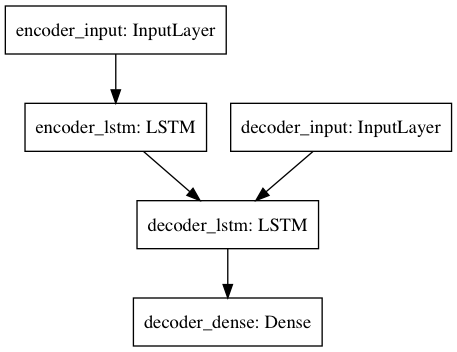
\includegraphics[width=0.5\linewidth]{img/draw-model6.png}
  \caption{Arquitetura Encoder-Decoder Desenvolvida}
  \label{fig:encdec}
\end{figure}

%ref[].

\subsection{Modelo Encoder-Decoder 1} 

\subsubsection{Corpus}
O modelo \textbf{Encoder-Decoder 1} foi treinado na base apresentada na Seção \ref{sec:corpus-ffd}, porém sem qualquer balanceamento relativo às proporções de verbos irregulares.

\subsubsection{Hiperparâmetros} 

\begin{table}[H]
\centering
\begin{tabular}{ll}
Numero de Amostras Treinamento: & 325 \\
Numero de Amostras Teste: & 100 \\
Numero de tokens unicos do Input: & 22 \\
Numero de tokens unicos do Output: & 26 \\
Comprimento maximo da sequencia para inputs: & 11 \\
Comprimento maximo da sequencia para outputs: & 13 \\
Loss: & categorical\_crossentropy \\
Optimizer & rmsprop \\
Activation & softmax \\
Epochs & 130 \\
Batch Size & 64
\end{tabular}
\caption{Tabela Resumo Estrutural do Modelo Encoder-Decoder 1}
\label{tab:res1}
\end{table}

\subsubsection{Resultados}

\begin{figure}[H]
  \centering
  \begin{subfigure}[b]{0.45\linewidth}
    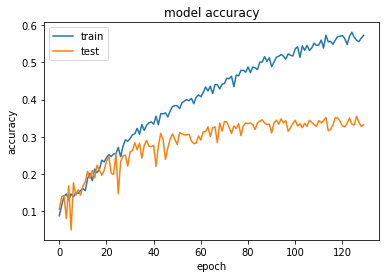
\includegraphics[width=\linewidth]{img/enc-dec-1.png}
    \caption{Resultados de Acurácia por Época}
  \end{subfigure}
  \begin{subfigure}[b]{0.45\linewidth}
    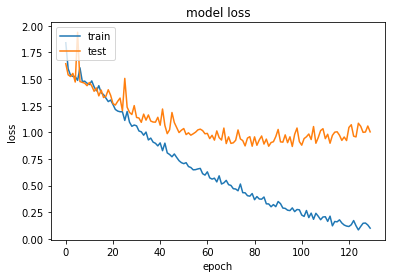
\includegraphics[width=\linewidth]{img/enc-dec-1-loss.png}
    \caption{Resultados de Custo por Época}
  \end{subfigure}
  \caption{Gráficos dos Resultados do Modelo}
  \label{fig:plots1}
\end{figure}

\begin{table}[H]
\centering
\begin{tabular}{llllll}
\textbf{Best Epoch Score} & \textbf{Val\_Acc} & \textbf{Vall\_Loss} & \textbf{Loss} & \textbf{Acc} & \textbf{Time} \\
97 & 0.342 & 0.867 & 0.290 & 0.508 & 2 min
\end{tabular}
\caption{Scores do Modelo Encoder-Decoder 1}
\label{tab:res-enc-dec-1}
\end{table}

\subsection{Modelo Encoder-Decoder 2}

\subsubsection{Corpus}
O modelo \textbf{Encoder-Decoder 2} foi treinado na base apresentada na Seção \ref{sec:corpus-ffd}, para o caso de proporção de 55\% de verbos irregulares. 

\subsubsection{Hiperparâmetros} 

\begin{table}[H]
\centering
\begin{tabular}{ll}
Numero de Amostras Treinamento: & 452 \\
Numero de Amostras Teste: & 21 \\
Numero de tokens unicos do Input: & 23 \\
Numero de tokens unicos do Output: & 27 \\
Comprimento maximo da sequencia para inputs: & 13 \\
Comprimento maximo da sequencia para outputs: & 15 \\
Loss: & categorical\_crossentropy \\
Optimizer & rmsprop \\
Activation & softmax \\
Epochs & 150 \\
Batch Size & 64
\end{tabular}
\caption{Tabela Resumo Estrutural do Modelo Encoder-Decoder 2}
\label{tab:res1}
\end{table}

\subsubsection{Resultados}

\begin{figure}[H]
  \centering
  \begin{subfigure}[b]{0.45\linewidth}
    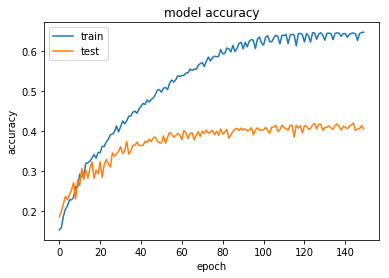
\includegraphics[width=\linewidth]{img/enc-dec-2.png}
    \caption{Resultados de Acurácia por Época}
  \end{subfigure}
  \begin{subfigure}[b]{0.45\linewidth}
    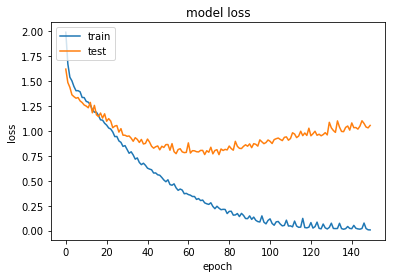
\includegraphics[width=\linewidth]{img/enc-dec-2-loss.png}
    \caption{Resultados de Custo por Época}
  \end{subfigure}
  \caption{Gráficos dos Resultados do Modelo}
  \label{fig:plots2}
\end{figure}

\begin{table}[H]
\centering
\begin{tabular}{llllll}
\textbf{Best Epoch Score} & \textbf{Val\_Acc} & \textbf{Vall\_Loss} & \textbf{Loss} & \textbf{Acc} & \textbf{Time} \\
145 & 0.419 & 1.048 & 0.014 & 0.644 & 4 min
\end{tabular}
\caption{Scores do Modelo Encoder-Decoder 2}
\label{tab:res-enc-dec-2}
\end{table}

\subsection{Modelo Encoder-Decoder 3}
 
\subsubsection{Corpus}

O corpus utilizado para o treinamento das redes \textbf{Encoder-Decoder 3}, \textbf{Encoder-Decoder 4} e \textbf{Encoder-Decoder 5}  foi baseado na lista de verbos disponíveis no site \url{https://www.conjugacao.com.br/verbos-populares/}.\\

As informações contidas nessa página diferem-se das páginas apresentadas na Seção \ref{sec:corpus-ffd} no sentido de que, em primeiro lugar, não há qualquer divisão entre verbos regulares ou irregulares (o que dificulta a segmentação manual dos verbos em diferentes famílias); apesar disso, ganha-se ao aumentar em quase cem vezes o tamanho da base de treino. 

Assim como na Seção \ref{sec:corpus-ffd}, foi realizada uma etapa de extração dos verbos e suas respectivas conjugações para um banco de dados local. Em seguida, os verbos foram mantidos em notação ortográfica como um exercício de prova de conceito. O objetivo dos testes que se seguem é avaliar o potencial preditivo quando se pode contar com uma base de treinamento consideravelmente maior. Perde-se pela considerável redução de resolução com relação ao reconhecimento de padrões fonológicos, fato que será discutido na Seção \ref{sec:disc}

\subsubsection{Hiperparâmetros} 

\begin{table}[H]
\centering
\begin{tabular}{ll}
Numero de Amostras Treinamento: & 2000 \\
Numero de Amostras Teste: & 100 \\
Numero de tokens unicos do Input: & 26 \\
Numero de tokens unicos do Output: & 32 \\
Comprimento maximo da sequencia para inputs: & 15 \\
Comprimento maximo da sequencia para outputs: & 16 \\
Loss: & categorical\_crossentropy \\
Optimizer & rmsprop \\
Activation & softmax \\
Epochs & 100 \\
Batch Size & 64
\end{tabular}
\caption{Tabela Resumo Estrutural do Modelo Encoder-Decoder 3}
\label{tab:res3}
\end{table}

\subsubsection{Resultados}
%falar q eu adicionei dropout e explicar oq é isso

\begin{figure}[H]
  \centering
  \begin{subfigure}[b]{0.45\linewidth}
    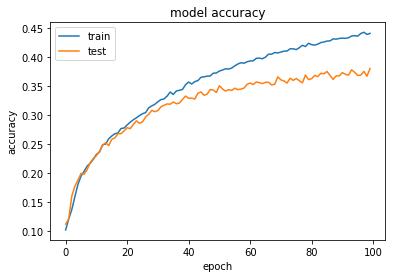
\includegraphics[width=\linewidth]{img/enc-dec-3.png}
    \caption{Resultados de Acurácia por Época}
  \end{subfigure}
  \begin{subfigure}[b]{0.45\linewidth}
    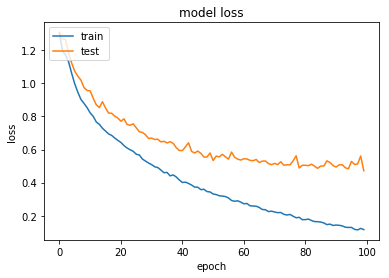
\includegraphics[width=\linewidth]{img/enc-dec-3-loss.png}
    \caption{Resultados de Custo por Época}
  \end{subfigure}
  \caption{Gráficos dos Resultados do Modelo}
  \label{fig:plots3}
\end{figure}

\begin{table}[H]
\centering
\begin{tabular}{llllll}
\textbf{Best Epoch Score} & \textbf{Val\_Acc} & \textbf{Vall\_Loss} & \textbf{Loss} & \textbf{Acc} & \textbf{Time} \\
100 & 0.380 & 0.471 & 0.115 & 0.440 & 11 min
\end{tabular}
\caption{Scores do Modelo Encoder-Decoder 3}
\label{tab:res-enc-dec-3}
\end{table}

\subsection{Modelo Encoder-Decoder 4}
%Falar que eu quis mudar a funcao de ativacao pra ver oq acontecia e o otimizador tb (deve ter tido uma razao pra eu ter feito isso, deve ta no deep learning la)

\subsubsection{Hiperparâmetros} 

\begin{table}[H]
\centering
\begin{tabular}{ll}
Numero de Amostras Treinamento: & 2000 \\
Numero de Amostras Teste: & 100 \\
Numero de tokens unicos do Input: & 26 \\
Numero de tokens unicos do Output: & 29 \\
Comprimento maximo da sequencia para inputs: & 15 \\
Comprimento maximo da sequencia para outputs: & 16 \\
Loss: & categorical\_crossentropy \\
Optimizer & adam \\
Activation & relu \\
Epochs & 100 \\
Batch Size & 64
\end{tabular}
\caption{Tabela Resumo Estrutural do Modelo Encoder-Decoder 4}
\label{tab:res4}
\end{table}

\subsubsection{Resultados}
%falar q eu adicionei dropout e explicar oq é isso

\begin{figure}[H]
  \centering
  \begin{subfigure}[b]{0.45\linewidth}
    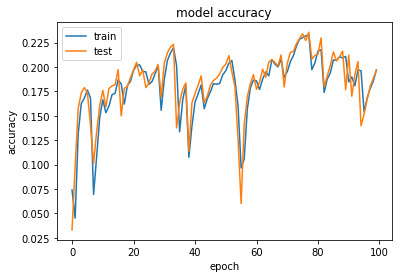
\includegraphics[width=\linewidth]{img/enc-dec-4.png}
    \caption{Resultados de Acurácia por Época}
  \end{subfigure}
  \begin{subfigure}[b]{0.45\linewidth}
    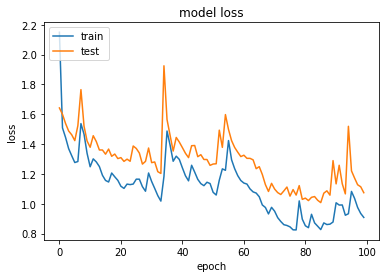
\includegraphics[width=\linewidth]{img/enc-dec-4-loss.png}
    \caption{Resultados de Custo por Época}
  \end{subfigure}
  \caption{Gráficos dos Resultados do Modelo}
  \label{fig:plots4}
\end{figure}

\begin{table}[H]
\centering
\begin{tabular}{llllll}
\textbf{Best Epoch Score} & \textbf{Val\_Acc} & \textbf{Vall\_Loss} & \textbf{Loss} & \textbf{Acc} & \textbf{Time} \\
86 & 0.210 & 1.00 & 0.820 & 0.207 & 10 min
\end{tabular}
\caption{Scores do Modelo Encoder-Decoder 4}
\label{tab:res-enc-dec-4}
\end{table}

 
 \subsection{Modelo Encoder-Decoder 5}
%Falar que eu quis aumentar mais ainda a amostra

\subsubsection{Hiperparâmetros} 

\begin{table}[H]
\centering
\begin{tabular}{ll}
Numero de Amostras Treinamento: & 3000 \\
Numero de Amostras Teste: & 100 \\
Numero de tokens unicos do Input: & 26 \\
Numero de tokens unicos do Output: & 32 \\
Comprimento maximo da sequencia para inputs: & 15 \\
Comprimento maximo da sequencia para outputs: & 16 \\
Loss: & categorical\_crossentropy \\
Optimizer & rmsprop \\
Activation & softmax \\
Epochs & 100 \\
Batch Size & 64
\end{tabular}
\caption{Tabela Resumo Estrutural do Modelo Encoder-Decoder 5}
\label{tab:res5}
\end{table}

\subsubsection{Resultados}
%falar q eu ainda nao adicionei o dropout mas pode ser legal adicionar

\begin{figure}[H]
  \centering
  \begin{subfigure}[b]{0.45\linewidth}
    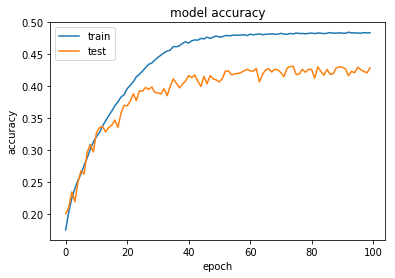
\includegraphics[width=\linewidth]{img/enc-dec-5.png}
    \caption{Resultados de Acurácia por Época}
  \end{subfigure}
  \begin{subfigure}[b]{0.45\linewidth}
    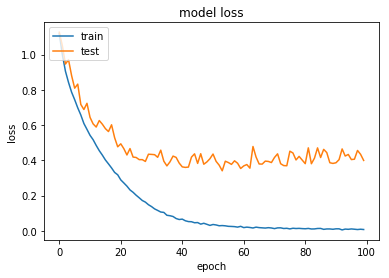
\includegraphics[width=\linewidth]{img/enc-dec-5-loss.png}
    \caption{Resultados de Custo por Época}
  \end{subfigure}
  \caption{Gráficos dos Resultados do Modelo}
  \label{fig:plots5}
\end{figure}

\begin{table}[H]
\centering
\begin{tabular}{llllll}
\textbf{Best Epoch Score} & \textbf{Val\_Acc} & \textbf{Vall\_Loss} & \textbf{Loss} & \textbf{Acc} & \textbf{Time} \\
54 & 0.423 & 0.340 & 0.030 & 0.4789 & 15 min
\end{tabular}
\caption{Scores do Modelo Encoder-Decoder 5}
\label{tab:res-enc-dec-5}
\end{table}

\section{Discussão}
\label{sec:disc}

Na Tabela \ref{tab:resultadosfdd} observa-se que aparentemente não há qualquer relação entre a proporção de verbos irregulares na base de treino e a acurácia do modelo. A acurácia foi cálculada a partir de uma base de teste em que considera-se um acerto apenas quando a sequência predita corresponde exatamente à sequência esperada. Apesar da variação percentual ser grande, os modelos podem ser considerados similares pois a base de teste era de apenas 21 verbos e uma predição incorreta de uma única conjugação significa uma perda de 4.76\% na acurácia. Tal variação pode ter ocorrido em decorrência da inicialização aleatória dos pesos. Com relação à métrica \textit{Loss}, observa-se que há alguma relação entre o aumento da proporção de verbos irregulares e a sua respectiva diminuição. Isso indica que a maior presença destes verbos ajudou, ainda que minimamente, na redução do erro quadrático médio. Essa redução não se converteu em ganho considerável de acurácia provavelmente pelo fato de que não houve aumento no número de exemplos distintos de verbos irregulares, somente no número de vezes que um mesmo verbo passou pelo treinamento. Isto pode ter provocado um \textit{underfitting} nos dados.

Os modelos Encoder-Decoder foram considerados principalmente pela independência das funções de decodificação para sequências. O cálculo recursivo a nível de caracter utilizando as LSTM's elimina o problema apontado na Seção \ref{sec:dec}. No entanto, como verificado nas figuras \ref{fig:plots1} e \ref{fig:plots2}, a grande distância entre a acurácia de treino e validação ainda indica \textit{underfitting}. Por essa razão, viu-se necessário o aumento da base de treino e o acréscimo de uma camada de \textit{Dropout}\footnote{Dropout é uma técnica de regularização que inativa aleatóriamente algumas unidades durante o treinamento. %ref
} = 0.25. Os resultados do modelo \textbf{Encoder-Decoder 3} (Fig. \ref{fig:plots3}) treinados em 2000 verbos distintos indicam redução notável na diferença entre os resultados obtidos para teste e validação. Ainda que tais resultados sejam inferiores aos obtidos pelos modelos \textbf{Encoder-Decoder 1} e \textbf{Encoder-Decoder 2}, deve-se lembrar que houve redução de resolução e acréscimo de features, uma vez que a base de treino é composta por verbos em notação ortográfica e não fonética. 

O modelo \textbf{Encoder-Decoder 4} foi desenvolvido com o objetivo de se testar uma diferente função de ativação. De acordo com %deeplearning tal tal
, sugere-se a utilização do otimizador "Adam" em conjunto com a função de ativação "RELU". Os resultados exibidos na Figura \ref{fig:plots4} demonstram um aprendizado completamente instável e fraco. 

Por último, o modelo \textbf{Encoder-Decoder 5} foi treinado em uma base de 3000 verbos distintos sem camada de Dropout e conseguiu o melhor resultado de acurácia (0.423) para o grupo de validação entre os modelos dessa mesma arquitetura. Com relação à outra arquitetura (FDD), a comparação torna-se de certa forma injusta pois, em primeiro lugar, a rede FDD é incapaz de gerar sequências maiores que quatro caracteres como discutido na Seção \ref{sec:dec}. Em segundo lugar, as bases de teste aplicadas são distintas: A base de teste da FFD é 30 vezes menor e é mais controlada com relação às irregularidades presentes.\\

Em resumo, os resultados obtidos até agora indicam que: 

\begin{enumerate}
\item Aumentar a base de treino parece aprimorar o aprendizado de forma significativa;
\item Aumentar o grau de resolução para transcrição fonética nessa mesma base pode aprimorar o aprendizado ainda mais (como observado nos resultados do modelo Encoder-Decoder 2);
\item O acréscimo da camada de Dropout surtiu um efeito muito interessante e a combinação com os demais itens apontados pode contribuir ainda mais para o aprimoramento do modelo.
\end{enumerate}

%\textit{1. Aumentar a base de treino parece aprimorar o treinamento de forma razoável}; \textit{2. Aumentar o grau de resolução para transcrição fonética nessa mesma base pode aprimorar o treinamento ainda mais (como observado nos resultados do modelo Encoder-Decoder 2)}; \textit{3. O acréscimo da camada de Dropout surtiu um efeito muito interessante e a combinação com os demais itens apontados pode contribuir ainda mais para o aprimoramento do modelo}.


\part{Próximos Passos}
\chapter{Próximos Passos}
\label{ch04:FutureSteps}


Os resultados obtidos até agora indicam que: \textit{1. Aumentar a base de treino parece aprimorar o treinamento de forma razoável}; \textit{2. Aumentar o grau de resolução para transcrição fonética nessa mesma base} 

In July we will present this work at one summer school organized by the company DeepMind in Europe \url{https://tmlss.ro/} and so we expect to gather more feedback on our research.

To address our research proposal we decided to formulate the following next steps:

\begin{itemize}
\item Apply regularization strategies on the available models to overcome the reported overfitting problem. 
\item Finish the Entailment-QA corpus to have a fine grain analysis of the result that we are seeing on the SICK corpus.
\item Explore the different extensions for all mentioned models.
\item Explore new models not mentioned here, like Dynamic Memory Networks \cite{KumarISBEPOGS15} and the models using the Memory Attention and Composition (MAC) cell \cite{Manning18}.
\item Create a visual version of the Entailment-QA to test logical inference with images.
\item There is a different literature that frames the dialog problem as an MDP (Markovian Decision Process) and a POMDP (Partially Observable Markovian Decision Process) applying different techniques of reinforcement learning (a recent example is \cite{Li:2016}). It is fruitful to investigate if these techniques can help our research.
\item One of the main focused here is model comparison. It would be fruitful if we could use the available literature  on the theory of comparing models (e.g.,  \cite{BenavoliCDZ17}) to refine our analysis.
\end{itemize}


\section{Cronograma}
\label{sec:work-plan}

Nesta seção, a tabela \ref{tab:schedule} serve de apoio visual para uma melhor compreensão sobre as atividades e objetivos realizados bem como atividades planejadas até o final do programa.

\begin{table}[ht!]
  \center
  \begin{tabular}{|c|c|c|c|c|}\hline
    {Atividade} & 2ºsem 2017 & 1ºsem 2018 & 2ºsem 2018 & 1ºsem 2019 \\ \hline \hline
    Disciplinas & \cellcolor{green!45} &\cellcolor{green!45} &  & \\ \hline
    Revisão Bibliográfica & \cellcolor{green!45} & \cellcolor{green!45} & \cellcolor{yellow!45} & \\ \hline 
    Modelagem Computacional & \cellcolor{green!45} & \cellcolor{green!45} & \cellcolor{yellow!45}& \\ \hline
    Publicações & & & \cellcolor{green!45} & \\ \hline
   Participação em Eventos da área &\cellcolor{green!45} & \cellcolor{green!45} & \cellcolor{yellow!45} & \cellcolor{orange!45}\\ \hline
    Escrita da Qualificação & &\cellcolor{green!45} &\cellcolor{green!45} &  \\ \hline
    Exame de Qualificação & & &\cellcolor{yellow!45} & \\ \hline
    Readequação de Corpus & & &\cellcolor{orange!45} &  \\ \hline
    Testes de Novos Modelos & & &\cellcolor{orange!45} &\\ \hline
    Testes Psico-linguísticos & & & &\cellcolor{orange!45} \\ \hline
    Análise Modelos Computacionais x Falantes & & & &\cellcolor{orange!45} \\ \hline
    Escrita Dissertação & & &\cellcolor{yellow!45} &\cellcolor{orange!45}\\ \hline
    Defesa & & & &\cellcolor{orange!45} \\ \hline
  \end{tabular}
  \caption{Cronograma. Atividades realizadas em verde, atividades sendo realizadas em amarelo e próximas atividades em laranja.}
  \label{tab:schedule}
\end{table}

\part{Apêndice}
\chapter{Apêndice}
\label{ch07:appendice}

\begin{figure}[H]
  \centering
  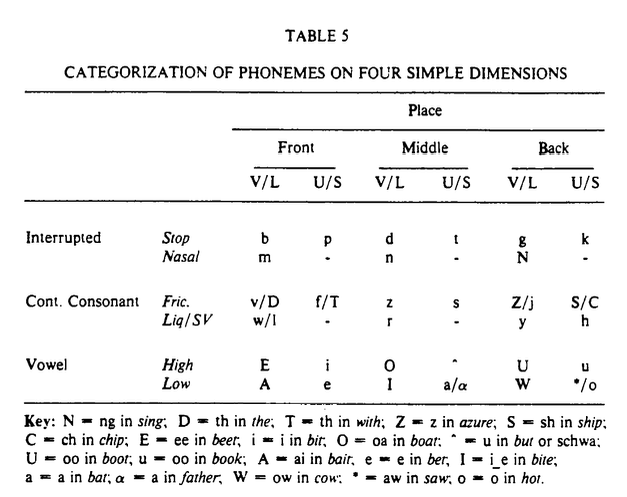
\includegraphics[width=0.5\linewidth]{img/Screen_Shot_2018-10-01_at_21_28_59.png}
  \caption{Tabela de Codificação de Rumelhart e McClelland}
  \label{fig:table-eng}
\end{figure}

% % cabeçalho para os apêndices
% \renewcommand{\chaptermark}[1]{\markboth{\MakeUppercase{\appendixname\ \thechapter}} {\MakeUppercase{#1}} }
% \fancyhead[RE,LO]{}
% \appendix

% \include{proofs}

% \include{ape-previous-work}

% ---------------------------------------------------------------------------- %
% Bibliografia
\backmatter \singlespacing   % espaçamento simples
\bibliographystyle{references-style-plainnat-ime} % citação bibliográfica textual
\bibliography{references}  % associado ao arquivo: 'bibliografia.bib'

% ---------------------------------------------------------------------------- %
% Índice remissivo
% \index{TBP|see{periodicidade região codificante}}
% \index{DSP|see{processamento digital de sinais}}
% \index{STFT|see{transformada de Fourier de tempo reduzido}}
% \index{DFT|see{transformada discreta de Fourier}}
% \index{Fourier!transformada|see{transformada de Fourier}}

% \printindex   % imprime o índice remissivo no documento 

\end{document}
